\documentclass[11pt]{article}
\usepackage[headheight=13.6pt,letterpaper, margin=1in]{geometry} % [letterpaper, margin=1in]
\usepackage[english]{babel}
\usepackage[utf8]{inputenc}
\usepackage{fancyhdr}
\usepackage{booktabs}
\usepackage{amsmath}
\usepackage{textcomp}
\usepackage{gensymb}
\usepackage{graphicx}
\usepackage{todonotes}
\usepackage{floatrow}
\usepackage{hyperref}
\usepackage{lastpage}

\newcommand\blfootnote[1]{%
  \begingroup
  \renewcommand\thefootnote{}\footnote{#1}%
  \addtocounter{footnote}{-1}%
  \endgroup
}

\def \hfillx {\hspace*{-\textwidth} \hfill}

\pagestyle{fancy}
\fancyhf{}
\rhead{Paras Jain // pjain67}
\lhead{CS4641 Project 4: Reinforcement Learning}
\cfoot{\thepage}

\title{CS4641: Reinforcement Learning}
\author{Paras Jain}
\date{}

\begin{document}

\maketitle

\begin{abstract}
This report details an exploration of Reinforcement Learning through \textit{Value Iteration}, \textit{Policy Iteration} and \textit{Q-Learning}. For interest of comparision, I also ran a short experiment using \textit{Prioritized Sweeping}. This paper compares Value Iteration and Policy Iteration to determine which situations each is best applicable. Tradeoffs between Value Iteration and Policy Iteration are explored. Analysis will conclude with a look at Q-learning and finally a brief comparision to Prioritized Sweeping.
\end{abstract}


% Come up with two interesting MDPs. Explain why they are interesting. They don't need to be overly complicated or directly grounded in a real situation, but it will be worthwhile if your MDPs are inspired by some process you are interested in or are familiar with. It's ok to keep it somewhat simple. For the purposes of this assignment, though, make sure one has a "small" number of states, and the other has a "large" number of states.
\section{Markov Decision Processes Chosen}
Two Markov decision processes were chosen of the same family of Gridworld MDPs (as covered in class). Two problems of the same class were chosen from the same class to compare how problem size affects.

The GridWorld MDP is where an agent is on a grid of squares and the goal is to reach some goal state. In order to encourage the agent to converge to a solution, there is a penalty of $-1$ for being in a state. Hitting a wall has a penalty of $-50$.

\subsection{Problem instances}

\begin{figure}[!htb]
    \begin{floatrow}
        \ffigbox{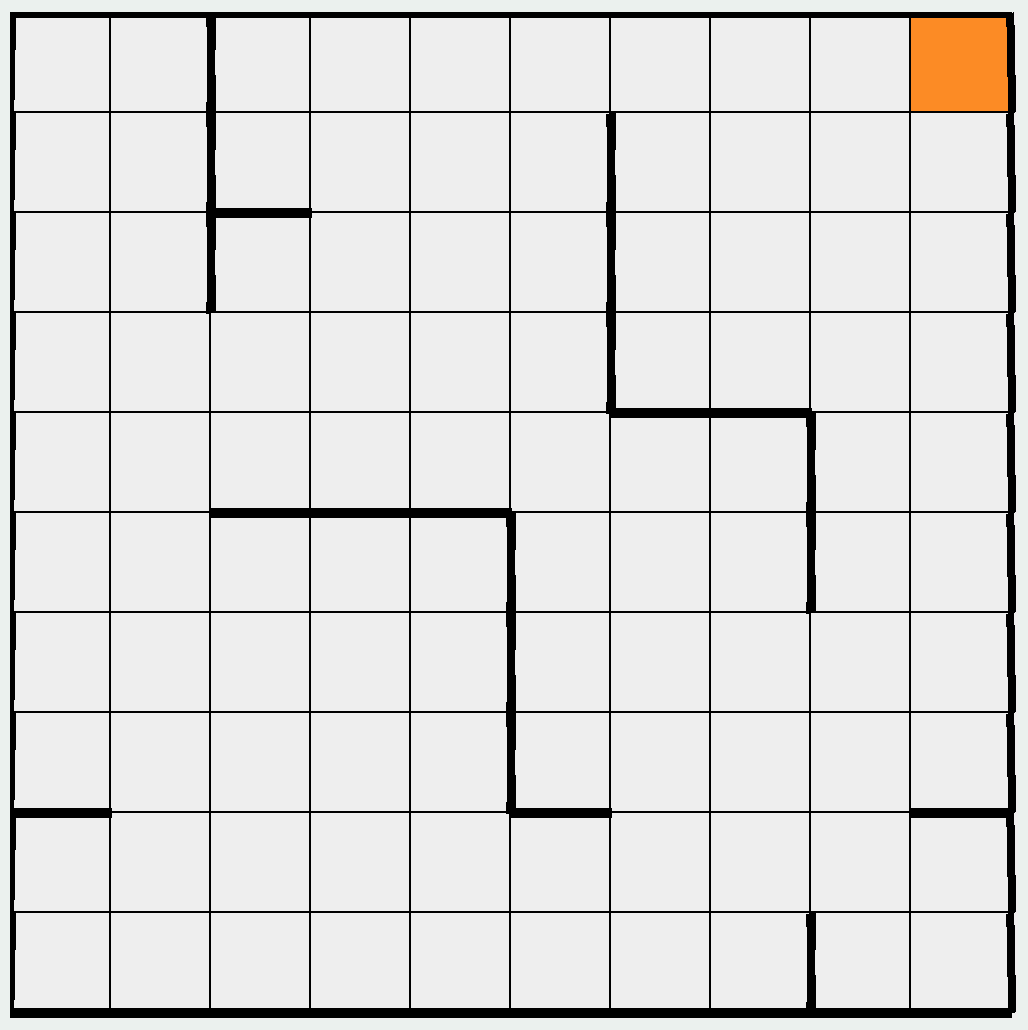
\includegraphics[width=.3\textwidth]{pics/medium}}{\centering\caption{Medium map. Goal state in orange.}\label{fig:mediummap}}
        \ffigbox{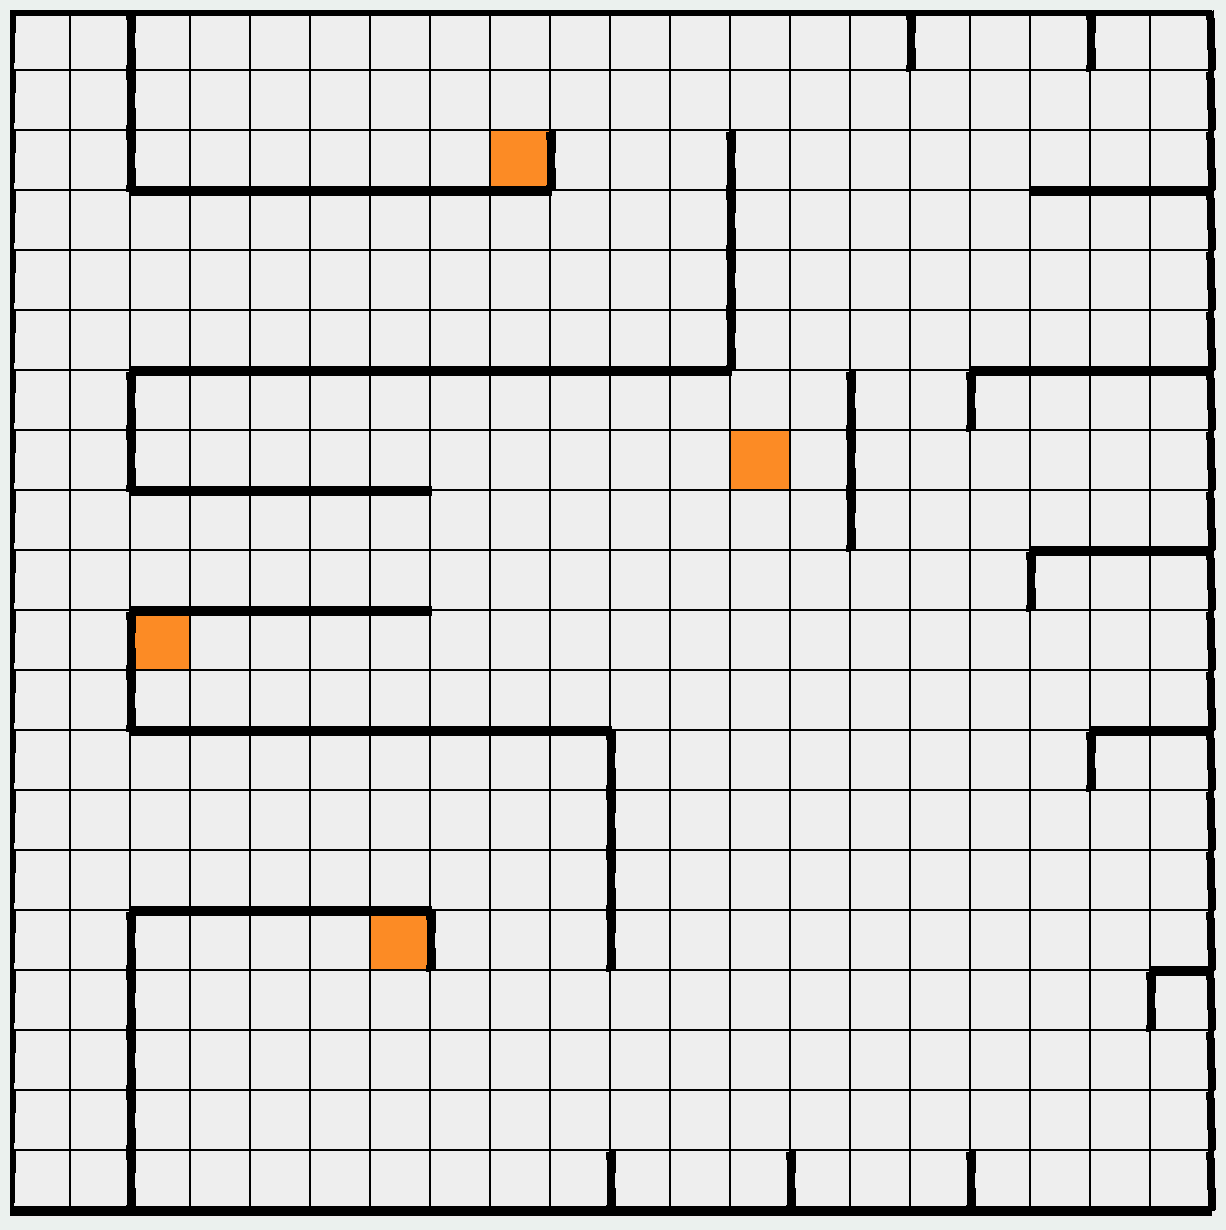
\includegraphics[width=.3\textwidth]{pics/big}}{\centering\caption{Large map. Goal state in orange.}\label{fig:bigmap}}
    \end{floatrow}
\end{figure}

Each state has a transition function Equation \ref{eq:mdptransition}, parametrized by probability $p$ which represents the probability of the transition not going as intended.

\begin{equation}
    \label{eq:mdptransition}
    S_{n+1}(x) = 
    \begin{cases}
        x,& \text{with probability } 1-p\\
        rotate(x, 90\degree),              & \text{with probability } \frac{p}{3}\\
        rotate(x, -90\degree),              & \text{with probability } \frac{p}{3}\\
        rotate(x, 180\degree),              & \text{with probability } \frac{p}{3}
    \end{cases}
\end{equation}

The medium map was designed to be relatively small with wide spaces with limited numbers of walls - refer to Figure \ref{fig:mediummap}. It is $10 \times 10$ with 100 total states. There is a single goal.

The large map was designed to have avenues with walls of varying configurations (varying length/width/direction avenues) - refer to Figure \ref{fig:bigmap}. It is $20 \times 20$ with 400 total states.

\subsection{MDP Interest}
I chose Gridworld as it is the most common example of reinforcement learning that students learn. The problem has received a huge amount of research attention and are relatively well understood. By choosing two instances of the same MDP class, we can compare the effect that board size has on the results.

For the large map, there are multiple goals in comparison to a single goal with the small map, which will be interesting to compare to the medium map. The placement of the goals is generally near walls which makes the direction of approach to a goal important. These walls make solving for an optimal policy much more difficult as there are channels through which the actor has to move through. These channels also will test exploration versus exploitation as if the agent does not explore enough, it will not navigate down the channel towards the goal.\footnote{See the Hallway Problem}

The multiple avenues should reveal some interesting conclusions regarding exploration versus exploitation. Note that there are various traps around some of the goals where some goal states are next to walls and corners which would make approaching the goals riskier than the goal in the open.




% Solve each MDP using value iteration as well as policy iteration. How many iterations does it take to converge? Which one converges faster? Why? Do they converge to the same answer? How did the number of states affect things, if at all?

\section{Phase 1 - Value Iteration/Policy Iteration}

\subsection{Value Iteration}

Refer to Table \ref{table:valueitertable}, Figure \ref{fig:valueiterationiterations} and Figure \ref{fig:valueiterationruntime} for results.

\begin{figure}[!h]
    \begin{floatrow}
        \ffigbox{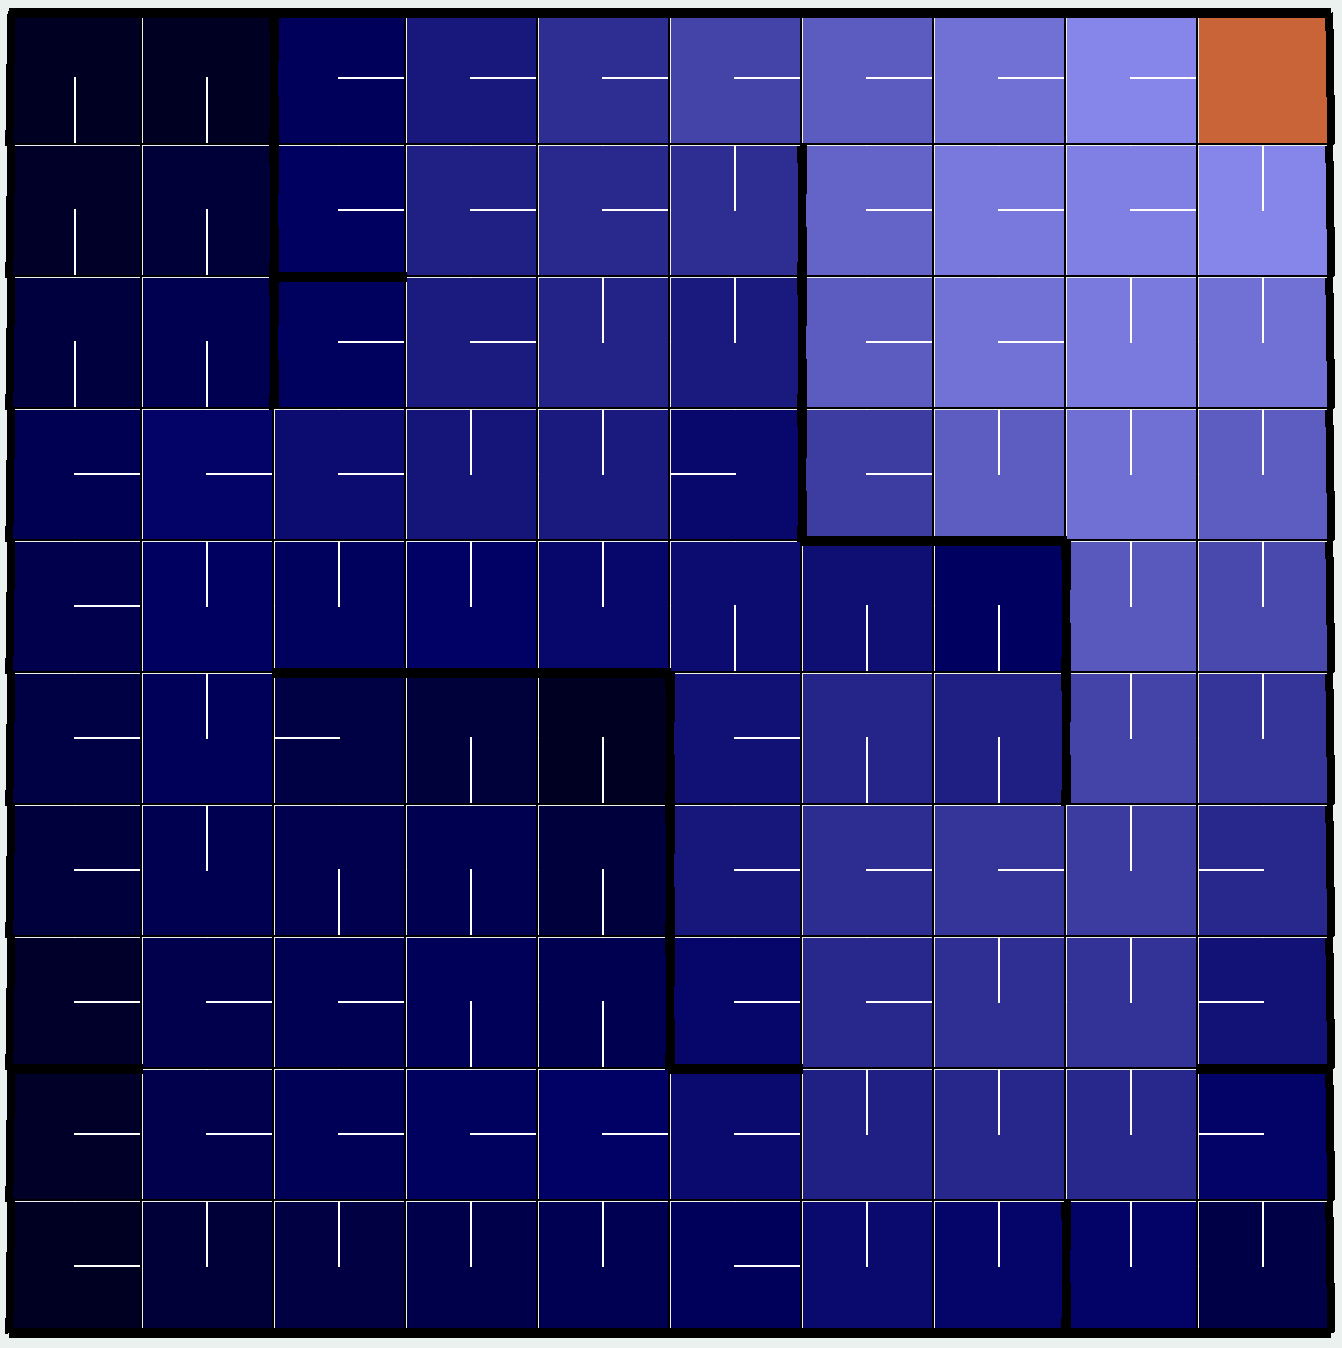
\includegraphics[width=.45\textwidth]{pics/value_iter_02}}{\caption{Value Iteration policy for medium map with $p=0.2$}\label{fig:valueiter02}}
        \ffigbox{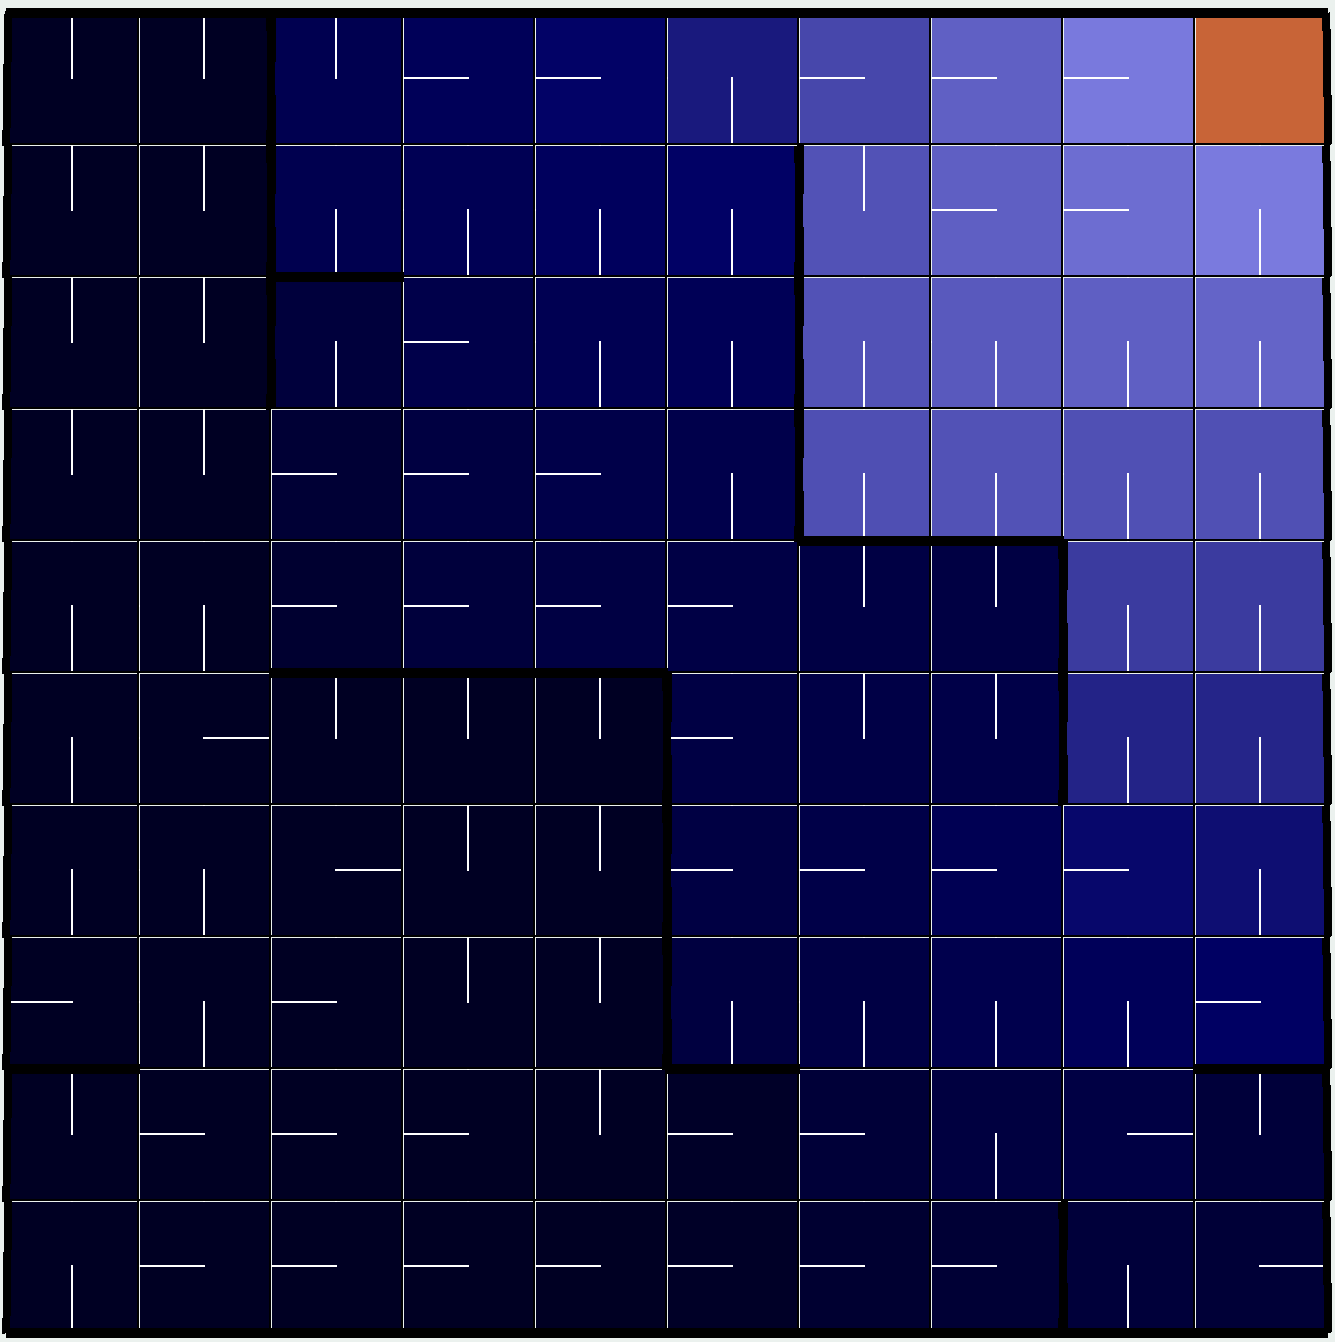
\includegraphics[width=.45\textwidth]{pics/value_iter_08}}{\caption{Value Iteration policy for medium map with $p=0.8$}\label{fig:valueiter08}}
    \end{floatrow}
\end{figure}
\begin{table}[!htb]
    \begin{minipage}{0.5\textwidth}
        \centering
        \textbf{Medium map}\\
        \begin{tabular}{@{}c|cc@{}}
        \toprule
        \textbf{$p$} & \textbf{Iterations} & \textbf{Time taken (ms)} \\ \midrule
        0.0          & 19                            & 51                       \\
        0.1          & 40                            & 20                       \\
        0.2          & 62                            & 29                       \\
        0.3          & 90                            & 48                       \\
        0.4          & 132                           & 85                       \\
        0.5          & 203                           & 89                       \\
        0.6          & 417                           & 196                      \\
        0.7          & 1821                          & 907                      \\
        0.8          & 2178                          & 1216                     \\
        0.9          & 679                           & 299                      \\
        1.0          & 708                           & 332                      \\ \bottomrule
        \end{tabular}
    \end{minipage}
    \hfillx
    \begin{minipage}{0.5\textwidth}
        \centering
        \textbf{Large map}\\
        \begin{tabular}{@{}c|cc@{}}
        \toprule
        \textbf{$p$} & \textbf{Iterations} & \textbf{Time taken (ms)} \\ \midrule
        0.0          & 18                  & 60                       \\
        0.1          & 37                  & 128                      \\
        0.2          & 54                  & 173                      \\
        0.3          & 80                  & 259                      \\
        0.4          & 127                 & 411                      \\
        0.5          & 193                 & 622                      \\
        0.6          & 420                 & 1397                     \\
        0.7          & 1503                & 5113                     \\
        0.8          & 1760                & 5910                     \\
        0.9          & 678                 & 2224                     \\
        1.0          & 471                 & 1560                     \\ \bottomrule
        \end{tabular}
    \end{minipage}
    \caption{Value iteration results for both maps. Note that $p$ is the probability of state transition error.}\label{table:valueitertable}
\end{table}
\begin{figure}[!htb]
    \begin{floatrow}
        \ffigbox{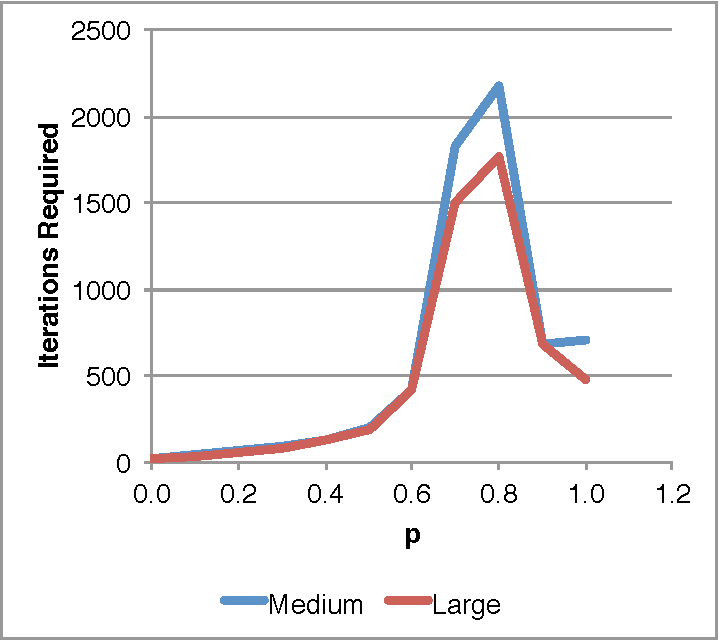
\includegraphics[width=.5\textwidth]{pics/ValueIterationIterations}}{\caption{Iterations to convergence for Value Iteration for both maps.}\label{fig:valueiterationiterations}}
        \ffigbox{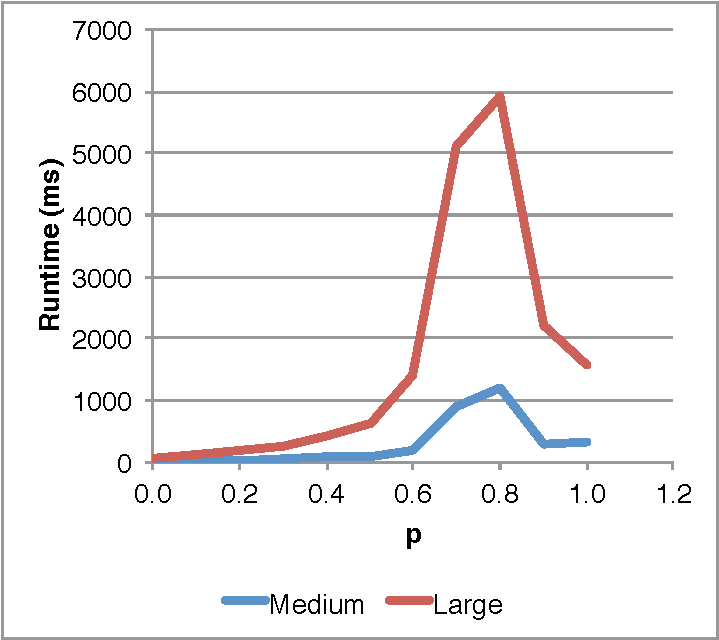
\includegraphics[width=.5\textwidth]{pics/ValueIterationRuntime}}{\caption{Runtime to convergence for Value Iteration for both maps.}\label{fig:valueiterationruntime}}
    \end{floatrow}
\end{figure}

Value iteration performed well on both gridworld problems. For value iteration, both runtime and steps taken were highly correlated to the value of $p$ in the MDP. Interestingly, the number of iterations to convergence was similar between the two map sizes. However, it appeared that the large map took significantly longer to converge than the medium map - this likely is just due to increased time taken per iteration which makes sense given that there are simply more states to process.

I suspect that the peak at $p = 0.8$ is because the transition model is essentially uniformly random across each of the 4 possible states. Optimizing this random behavior is understandably difficult, especially given how value iteration works.

Compare Figure \ref{fig:valueiter02} and Figure \ref{fig:valueiter08} to see how generated policies varied between $p=0.2$ and $p=0.8$. For $p=0.8$, the policy seems to avoid walls and then seems to generally choose the action that brings the agent closer to the goal. For $p=0.8$, it seems that the agent chooses to collide with walls and otherwise tries to escape from the goal. This seems to not make any sense but consider that the agent has a lower probability of successfully transitioning to the desired state than transitioning to an undesired state. As it is more confident that it will fail, value iteration chose to do the opposite action.

\subsection{Policy Iteration}

Refer to Table \ref{table:policyitertable}, Figure \ref{fig:policyiterationiterations} and Figure \ref{fig:policyiterationruntime} for results.

\begin{figure}[!h]
    \begin{floatrow}
        \ffigbox{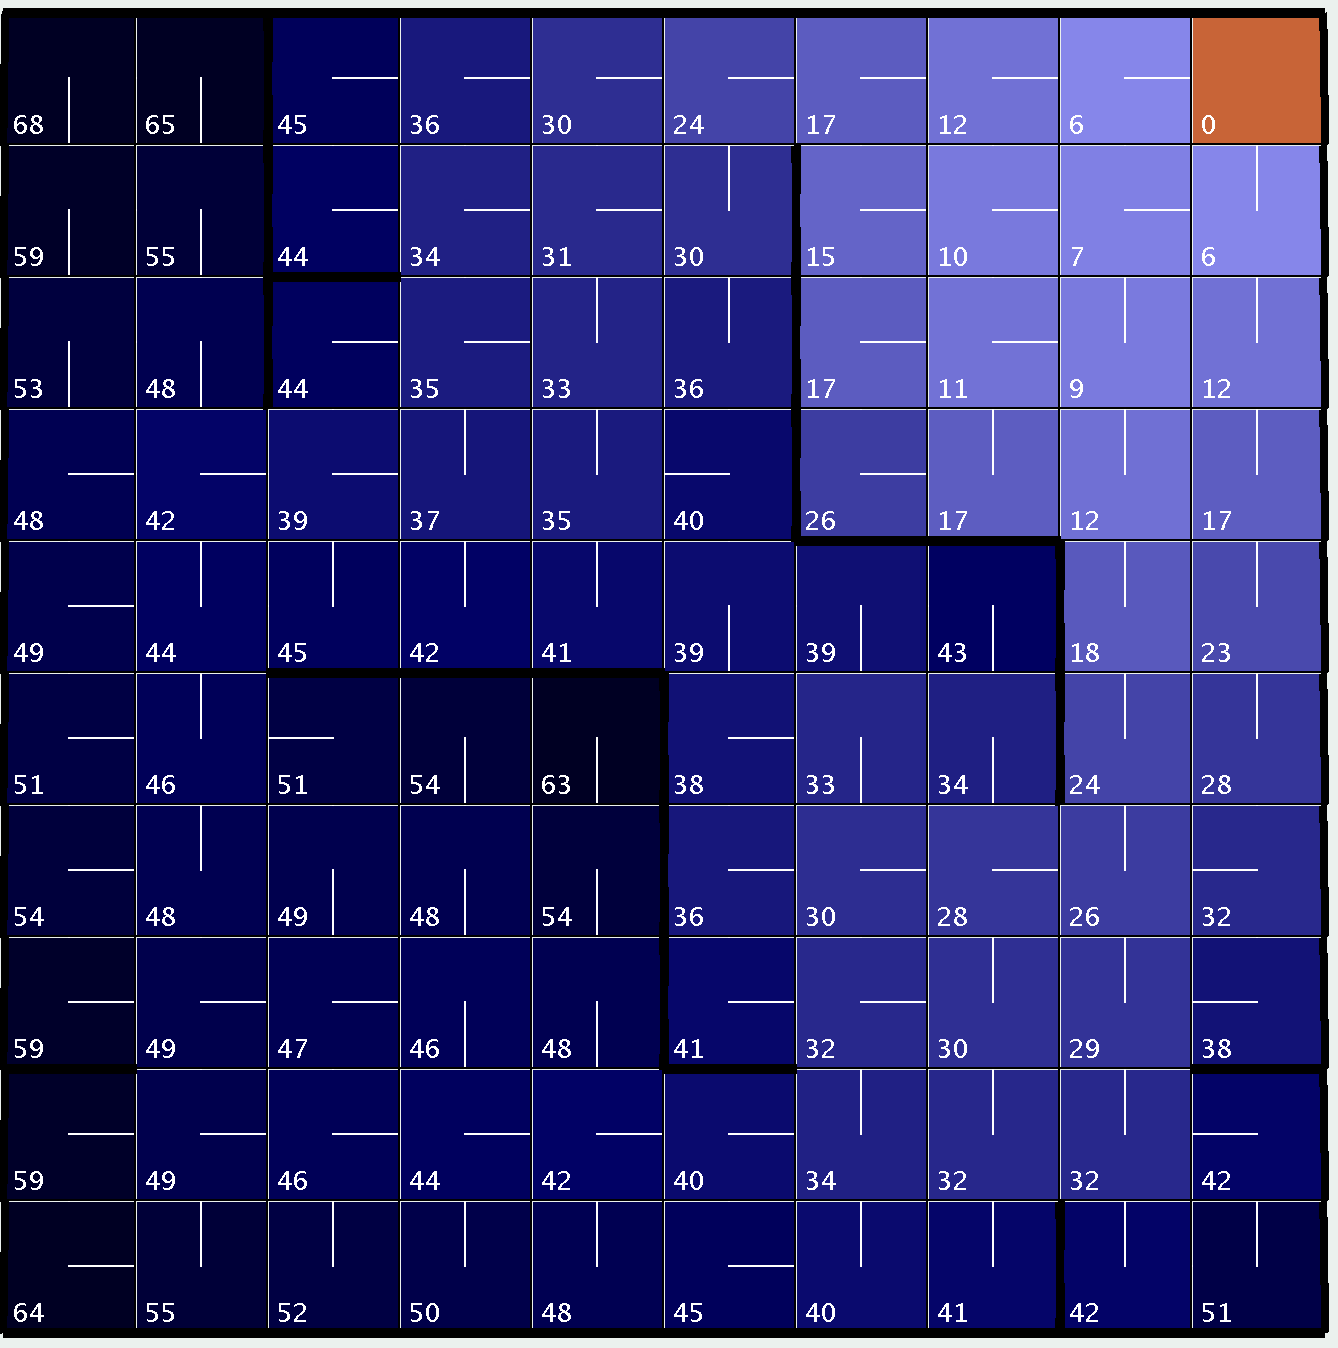
\includegraphics[width=.5\textwidth]{pics/policy_iter_02}}{\caption{Policy Iteration policy for medium map with $p=0.2$}\label{fig:policyiter02}}
        \ffigbox{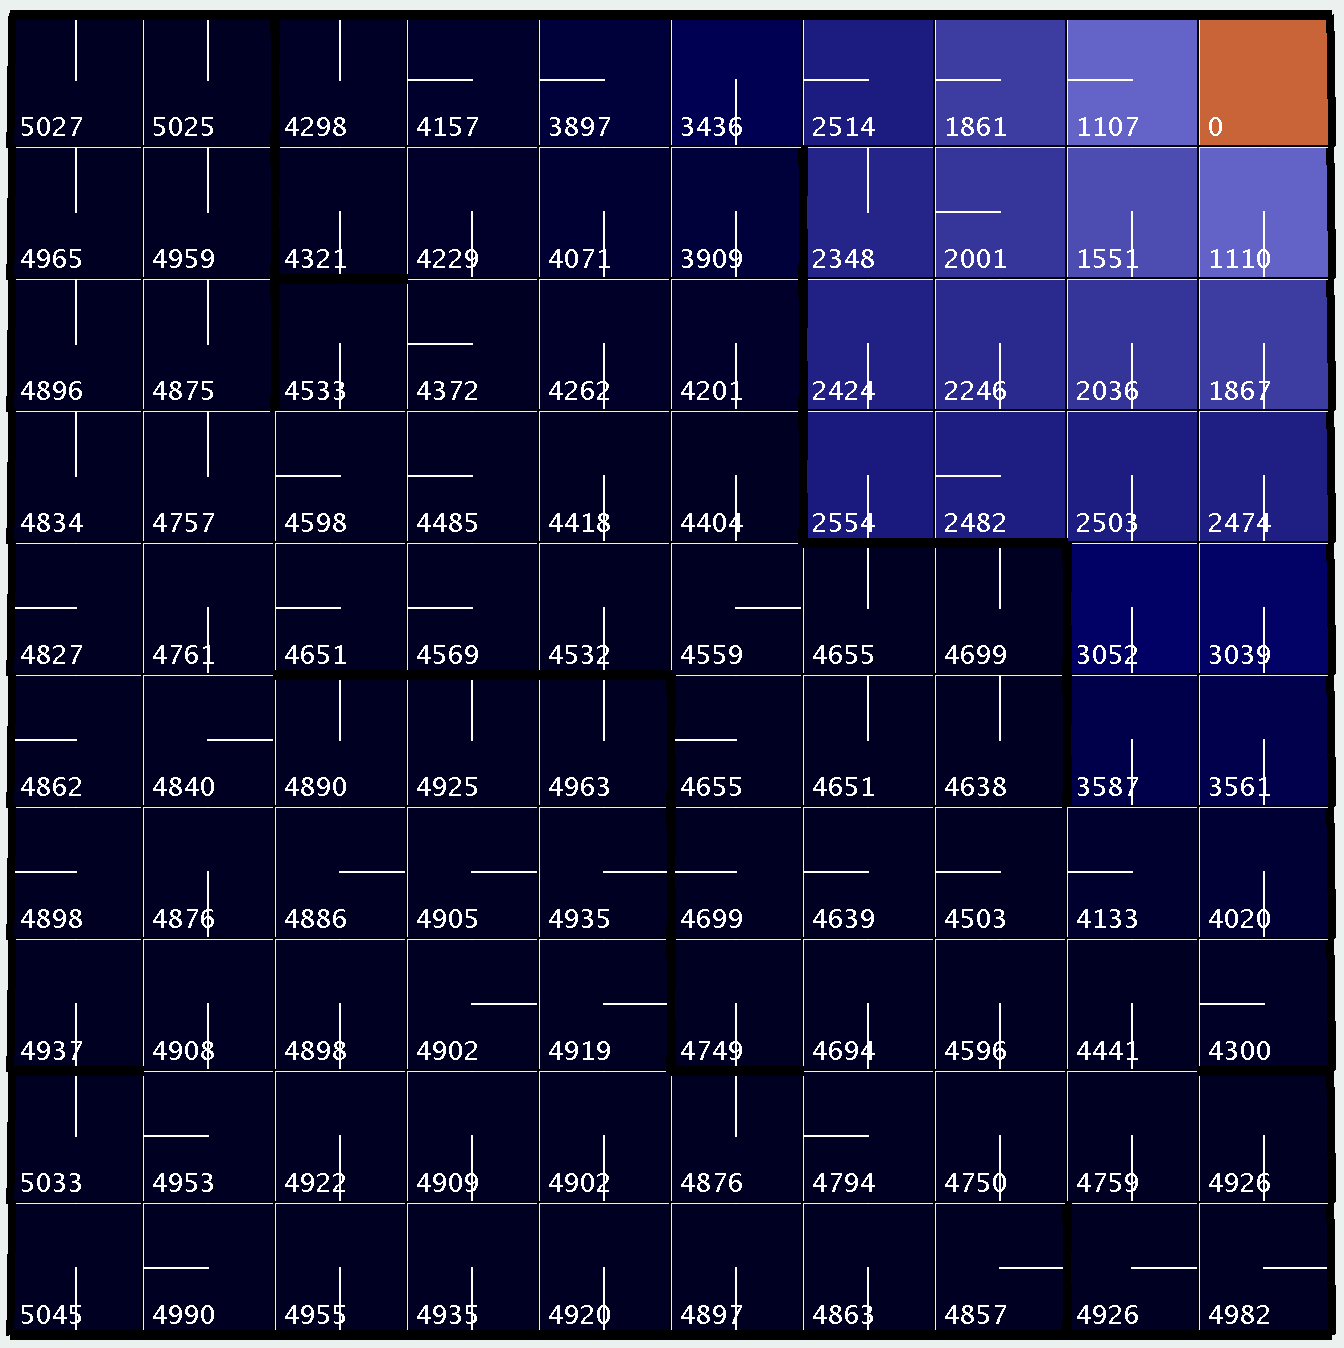
\includegraphics[width=.5\textwidth]{pics/policy_iter_08}}{\caption{Policy Iteration policy for medium map with $p=0.8$}\label{fig:policyiter08}}
    \end{floatrow}
\end{figure}
\begin{table}[!htb]
    \begin{minipage}{0.5\textwidth}
        \centering
        \textbf{Medium map}\\
        \begin{tabular}{@{}c|cc@{}}
        \toprule
        \textbf{$p$} & \textbf{Iterations} & \textbf{Time taken (ms)} \\ \midrule
        0.0     &   11      &    84  \\
        0.1     &   6       &    155  \\
        0.2     &   7       &    105  \\
        0.3     &   7       &    59  \\
        0.4     &   6       &    75  \\
        0.5     &   15      &    82  \\
        0.6     &   5       &    129  \\
        0.7     &   5       &    164  \\
        0.8     &   23      &    49  \\
        0.9     &   24      &    199  \\
        1.0     &   16      &    213  \\ \bottomrule
        \end{tabular}
    \end{minipage}
    \hfillx
    \begin{minipage}{0.5\textwidth}
        \centering
        \textbf{Large map}\\
        \begin{tabular}{@{}c|cc@{}}
        \toprule
        \textbf{$p$} & \textbf{Iterations} & \textbf{Time taken (ms)} \\ \midrule
        0.0     &    15      &   692  \\
        0.1     &    13      &   672  \\
        0.2     &    18      &   451  \\
        0.3     &    15      &   523  \\
        0.4     &    9       &   340  \\
        0.5     &    8       &   560  \\
        0.6     &    6       &   961  \\
        0.7     &    7       &   1310  \\
        0.8     &    57      &   1655  \\
        0.9     &    312     &   2888  \\
        1.0     &    18      &   1625  \\ \bottomrule
        \end{tabular}
    \end{minipage}
    \caption{Policy iteration results for both maps. Note that $p$ is the probability of state transition error.}\label{table:policyitertable}
\end{table}
\begin{figure}[!htb]
    \begin{floatrow}
        \ffigbox{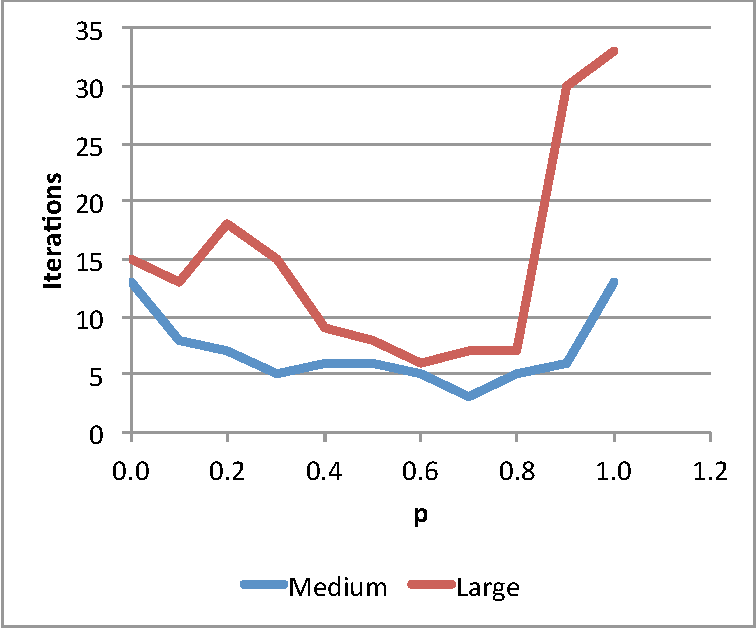
\includegraphics[width=.5\textwidth]{pics/PolicyIterationIterations}}{\caption{Iterations to convergence for Policy Iteration for both maps.}\label{fig:policyiterationiterations}}
        \ffigbox{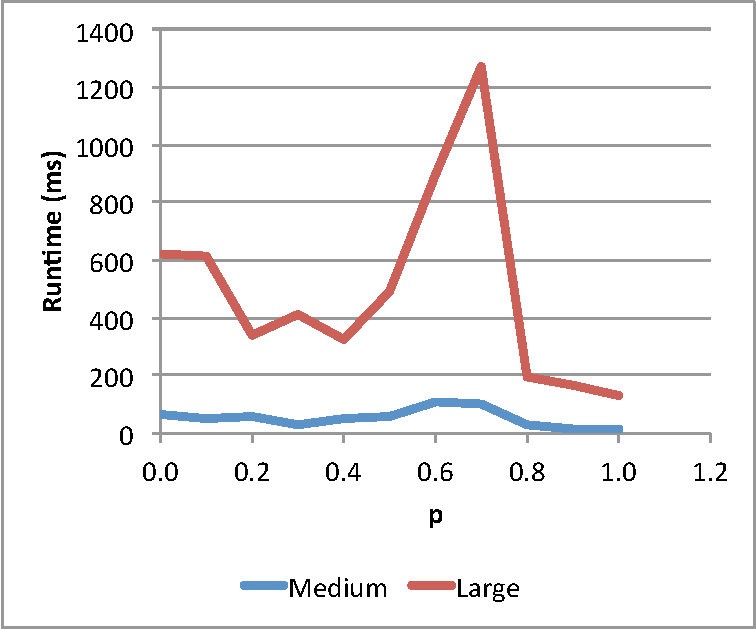
\includegraphics[width=.5\textwidth]{pics/PolicyIterationRuntime}}{\caption{Runtime to convergence for Policy Iteration for both maps.}\label{fig:policyiterationruntime}}
    \end{floatrow}
\end{figure}

Policy iteration seems to be much more stable across the choice of $p$ with exception with one outlier. The total number of iterations to convergence is much lower for policy iteration. Runtime also is similarly relatively stable with the exception of one outlier at $p=0.7$ for the large map. Iterations seemed to increase for values of $p$ close to 1. This makese sense as this would mean the agent almost never does the intended action. It is interesting to see that runtime was slightly higher for $p=0$ for the large map which meant that the agent always completed the intended action. Perhaps this is due to limited exploration in a exploration vs exploitation tradeoff where it rarely completed sub-optimal actions.

Compare Figure \ref{fig:policyiter02} and Figure \ref{fig:policyiter08} to see how generated policies varied between $p=0.2$ and $p=0.8$. For $p=0.2$, the results are relatively straightforward. $p=0.8$ generated an inverted policy where it seems to be taking a less probable sub-optimal action with the goal of obtaining a desired state transition. Like value iteration, policy iteration seemed to take advantage of this trick.


\subsection{Value iteration versus Policy Iteration}

Overall, policy iteration was significantly faster to run to convergence than value iteration for the Gridworld MDPs. It also appears to have fewer pathological cases of $p$ as compared to value iteration. When deciding which problem to use, consider how the problem domain scales - value iteration has better asymptotic runtime as compared to policy iteration (refer to Table \ref{table:valueitervspolicyiter}).

\begin{table}[]
\centering
\caption{Asymptotic behavior of algorithms explored by examining the percentage increase in runtime from the medium map to the large map.}
\label{table:valueitervspolicyiter}
\begin{tabular}{@{}cc@{}}
\toprule
\textbf{Algorithm} & \textbf{\% Increase in Runtime} \\ \midrule
Value Iteration    & 450\%                           \\
Policy Iteration   & 840\%                           \\ \bottomrule
\end{tabular}
\end{table}

Comparing generated policies (Figure \ref{fig:valueiter02} and Figure \ref{fig:valueiter08} versus Figure \ref{fig:policyiter02} and Figure \ref{fig:policyiter08}), both algorithms have very similar policies. Both algorithms were able to utilize the fact that attempting a low probability sub-optimal transition could result in an optimal transition.

Policy iteration appeared to take much fewer iterations to converge as compare to value iteration. Policy iteration does much more work in each iteration than value iteration which explains why it's runtime is not absurdly smaller than value iteration. Policy evaluation is expensive but it seems to be worth it as overall, policy iteration was faster than value iteration.

Comparing the algorithm performance as a function of $p$, value iteration is strong at situations where action is definite (either high $p$ or low $p$). Value iteration has pathological performance in situations where the transition state is very ambiguous. This makes Policy Iteration much better suited to situations where there is a non-negligible amount of noise (in say sensor readings or localization). I would suspect therefore that Policy Iteration would work much better for real-world RL robots. However, value iteration did produce more optimal solutions for extremely ambiguous transition models (about $p \gt 0.7$). This runtime-performance tradeoff is something to consider when choosing an algorithm with extreme amounts of noise.

This analysis aligns with the intuition that policy iteration is better for situations where the transition model is large with many possible actions. However, value iteration excels where the state space is large or grows non-linearly.\footnote{Consider gridworld where the states space grows at $O(n^2)$ where $n$ is the length of the grid}



% Now pick your favorite reinforcement learning algorithm and use it to solve the two MDPs. How does it perform, especially in comparison to the cases above where you knew the model, rewards, and so on? What exploration strategies did you choose? Did some work better than others?

\section{Phase 2 - Q-Learning and Prioritized Sweeping}

\subsection{Q-Learning}

\subsubsection{Parameter Hyperspace Analysis Experiment}

To study Q-learning, I modeled the parameter space to analyze the how parameters affected Q-learning. I explored a hyperspace of parameters, runtime and score. Out of some initial tests, I determined to focus analysis on a subset of parameters and the effect on two key performance metrics of a RL algorithm - runtime and utility achieved.

Iterations was fixed at 10,000 in this case in order to be able to visualize the highly-dimensional parameter space to produce meaningful conclusions. Some experiments were run over 20 trials with the results averaged in order to reduce the effect of randomization.

\subsubsection{Parameter Hyperspace Analysis Experiment Results}

Refer to Figure \ref{fig:qlscatter}\footnote{For an interactive 3D scatter plot, see \url{https://plot.ly/~parasj/4.embed}} and Figure \ref{fig:qlscatterbig}\footnote{\label{qlscatterbigsouce}For an interactive 3D scatter plot, see \url{https://plot.ly/~parasj/6.embed}} for visualization of the parameter space over $p$, $\epsilon$ and scores. Score in these charts is the value function where smaller values are better.

\begin{figure}[h]
    \begin{floatrow}
        \ffigbox{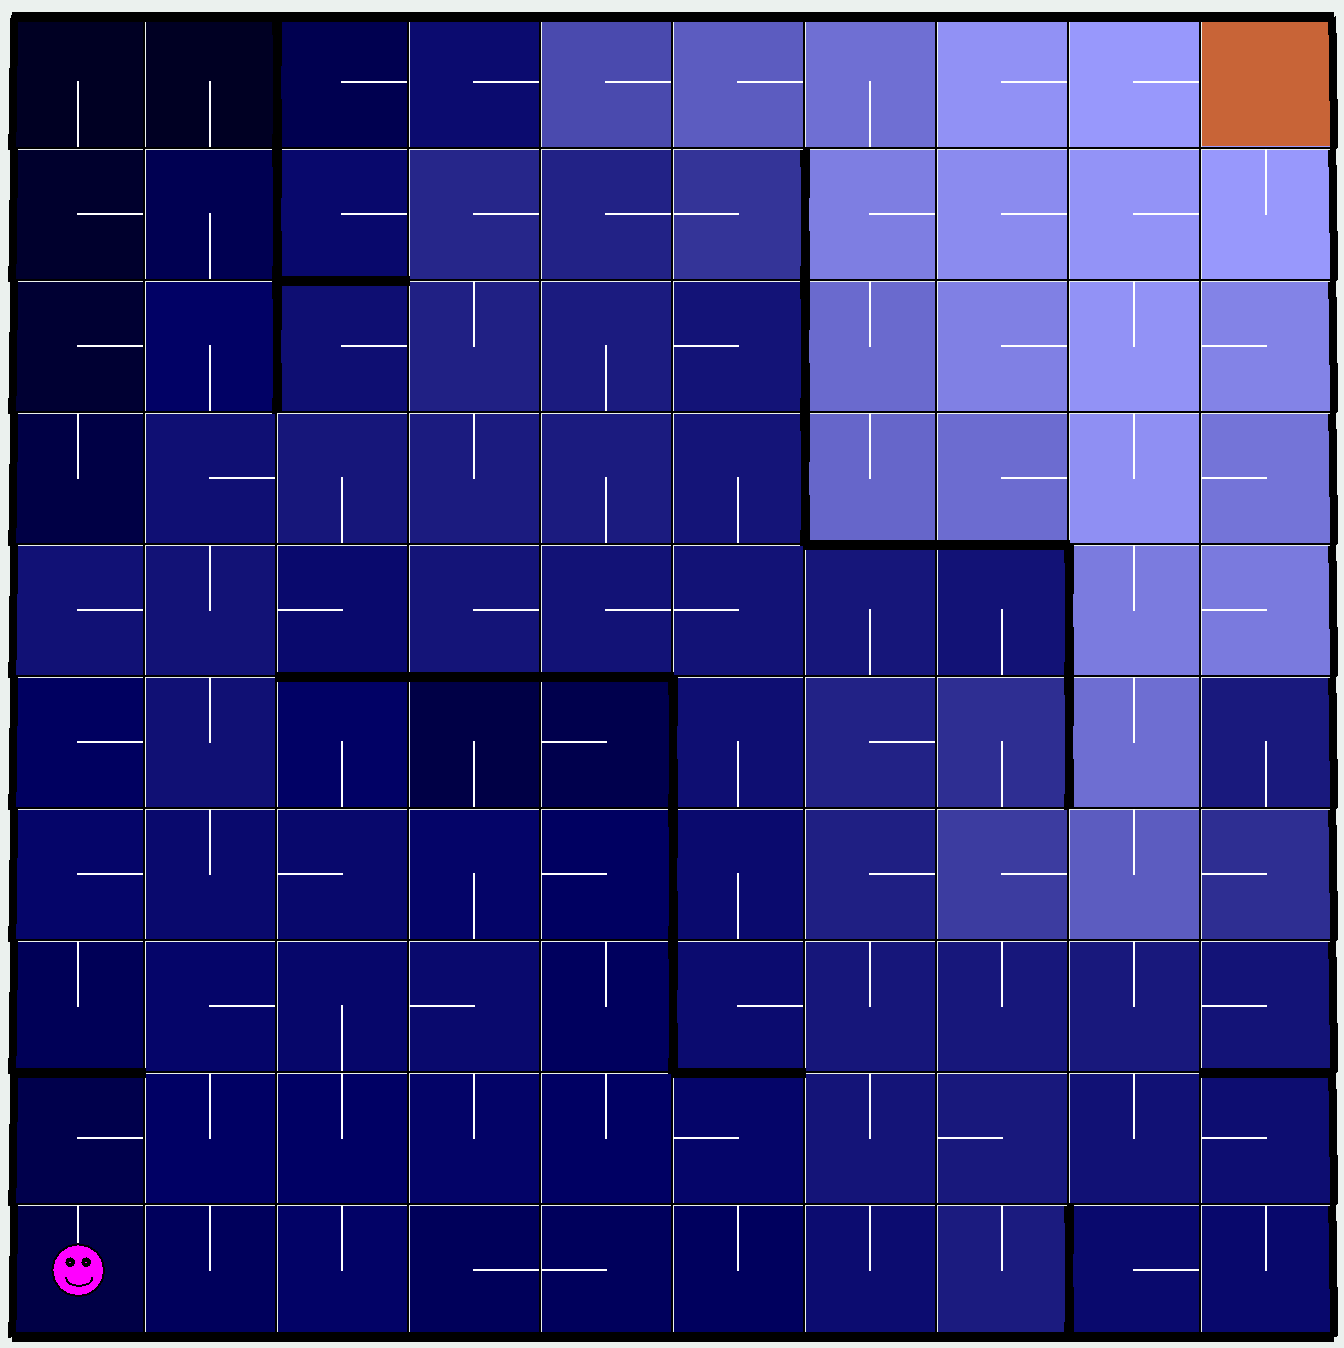
\includegraphics[width=.5\textwidth]{pics/qlearning_medium_03_01}}{\centering\caption{Q-learning policy after 10,000 iterations with $p=0.3$, $\epsilon=0.1$}\label{fig:qlpolicy0301}}
        \ffigbox{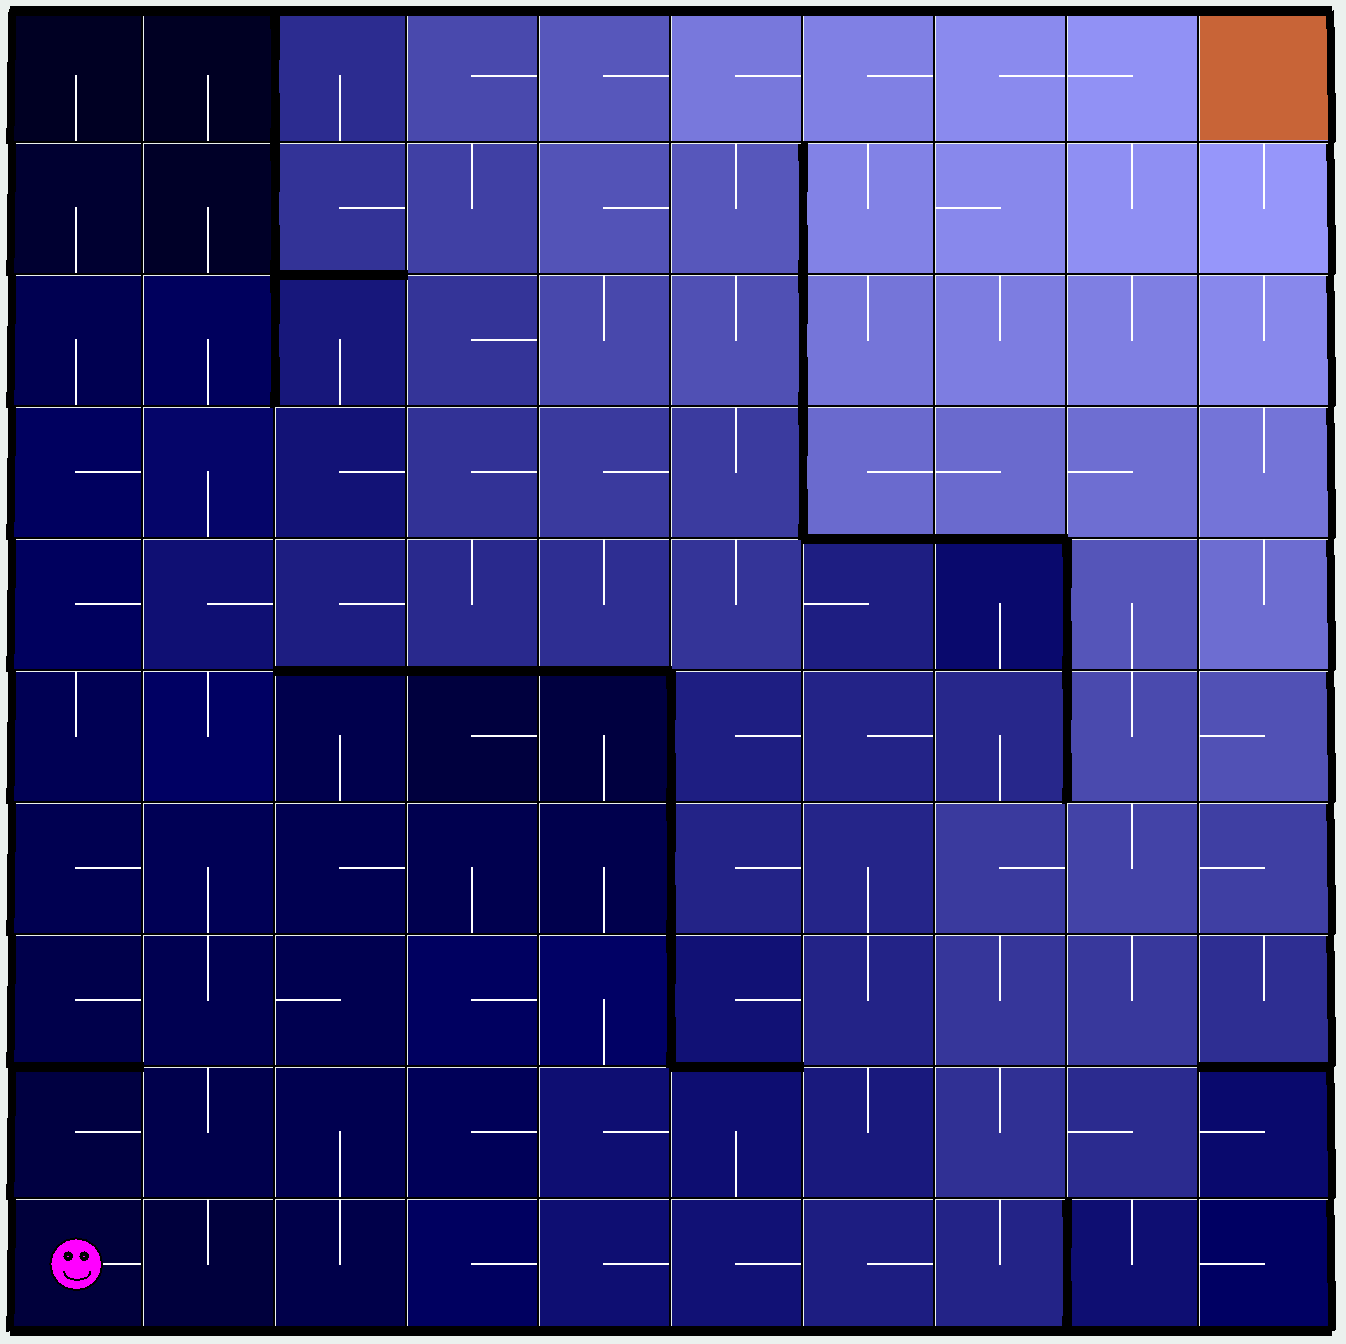
\includegraphics[width=.5\textwidth]{pics/qlearning_medium_07_01}}{\centering\caption{Q-learning policy after 10,000 iterations with $p=0.7$, $\epsilon=0.1$}\label{fig:qlpolicy0301}}
    \end{floatrow}
\end{figure}
\begin{figure}[!htb]
    \begin{floatrow}
        \ffigbox{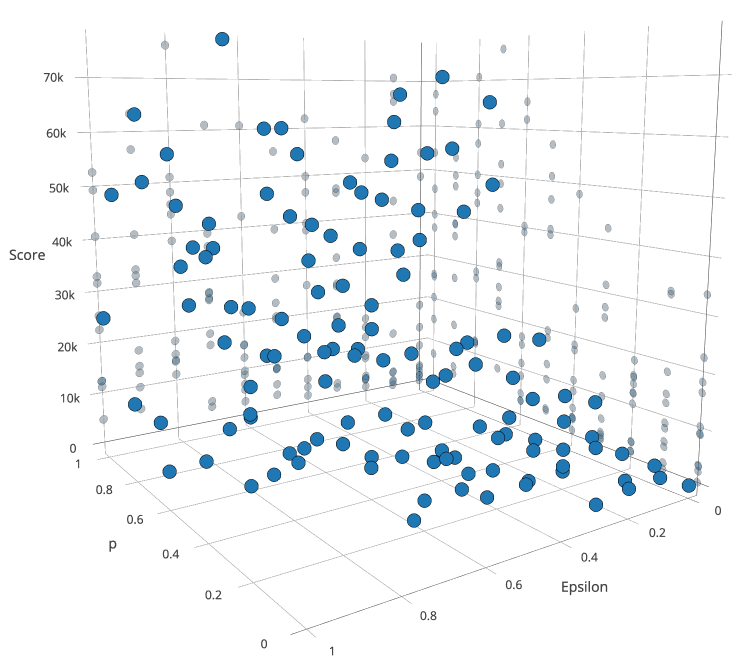
\includegraphics[width=.5\textwidth]{pics/medium03_scatter}}{\centering\caption{Q-Learning scores for the medium map over a space of $p$ and $\epsilon$ values, visualized as a 3D scatter plot.}\label{fig:qlscatter}}
        \ffigbox{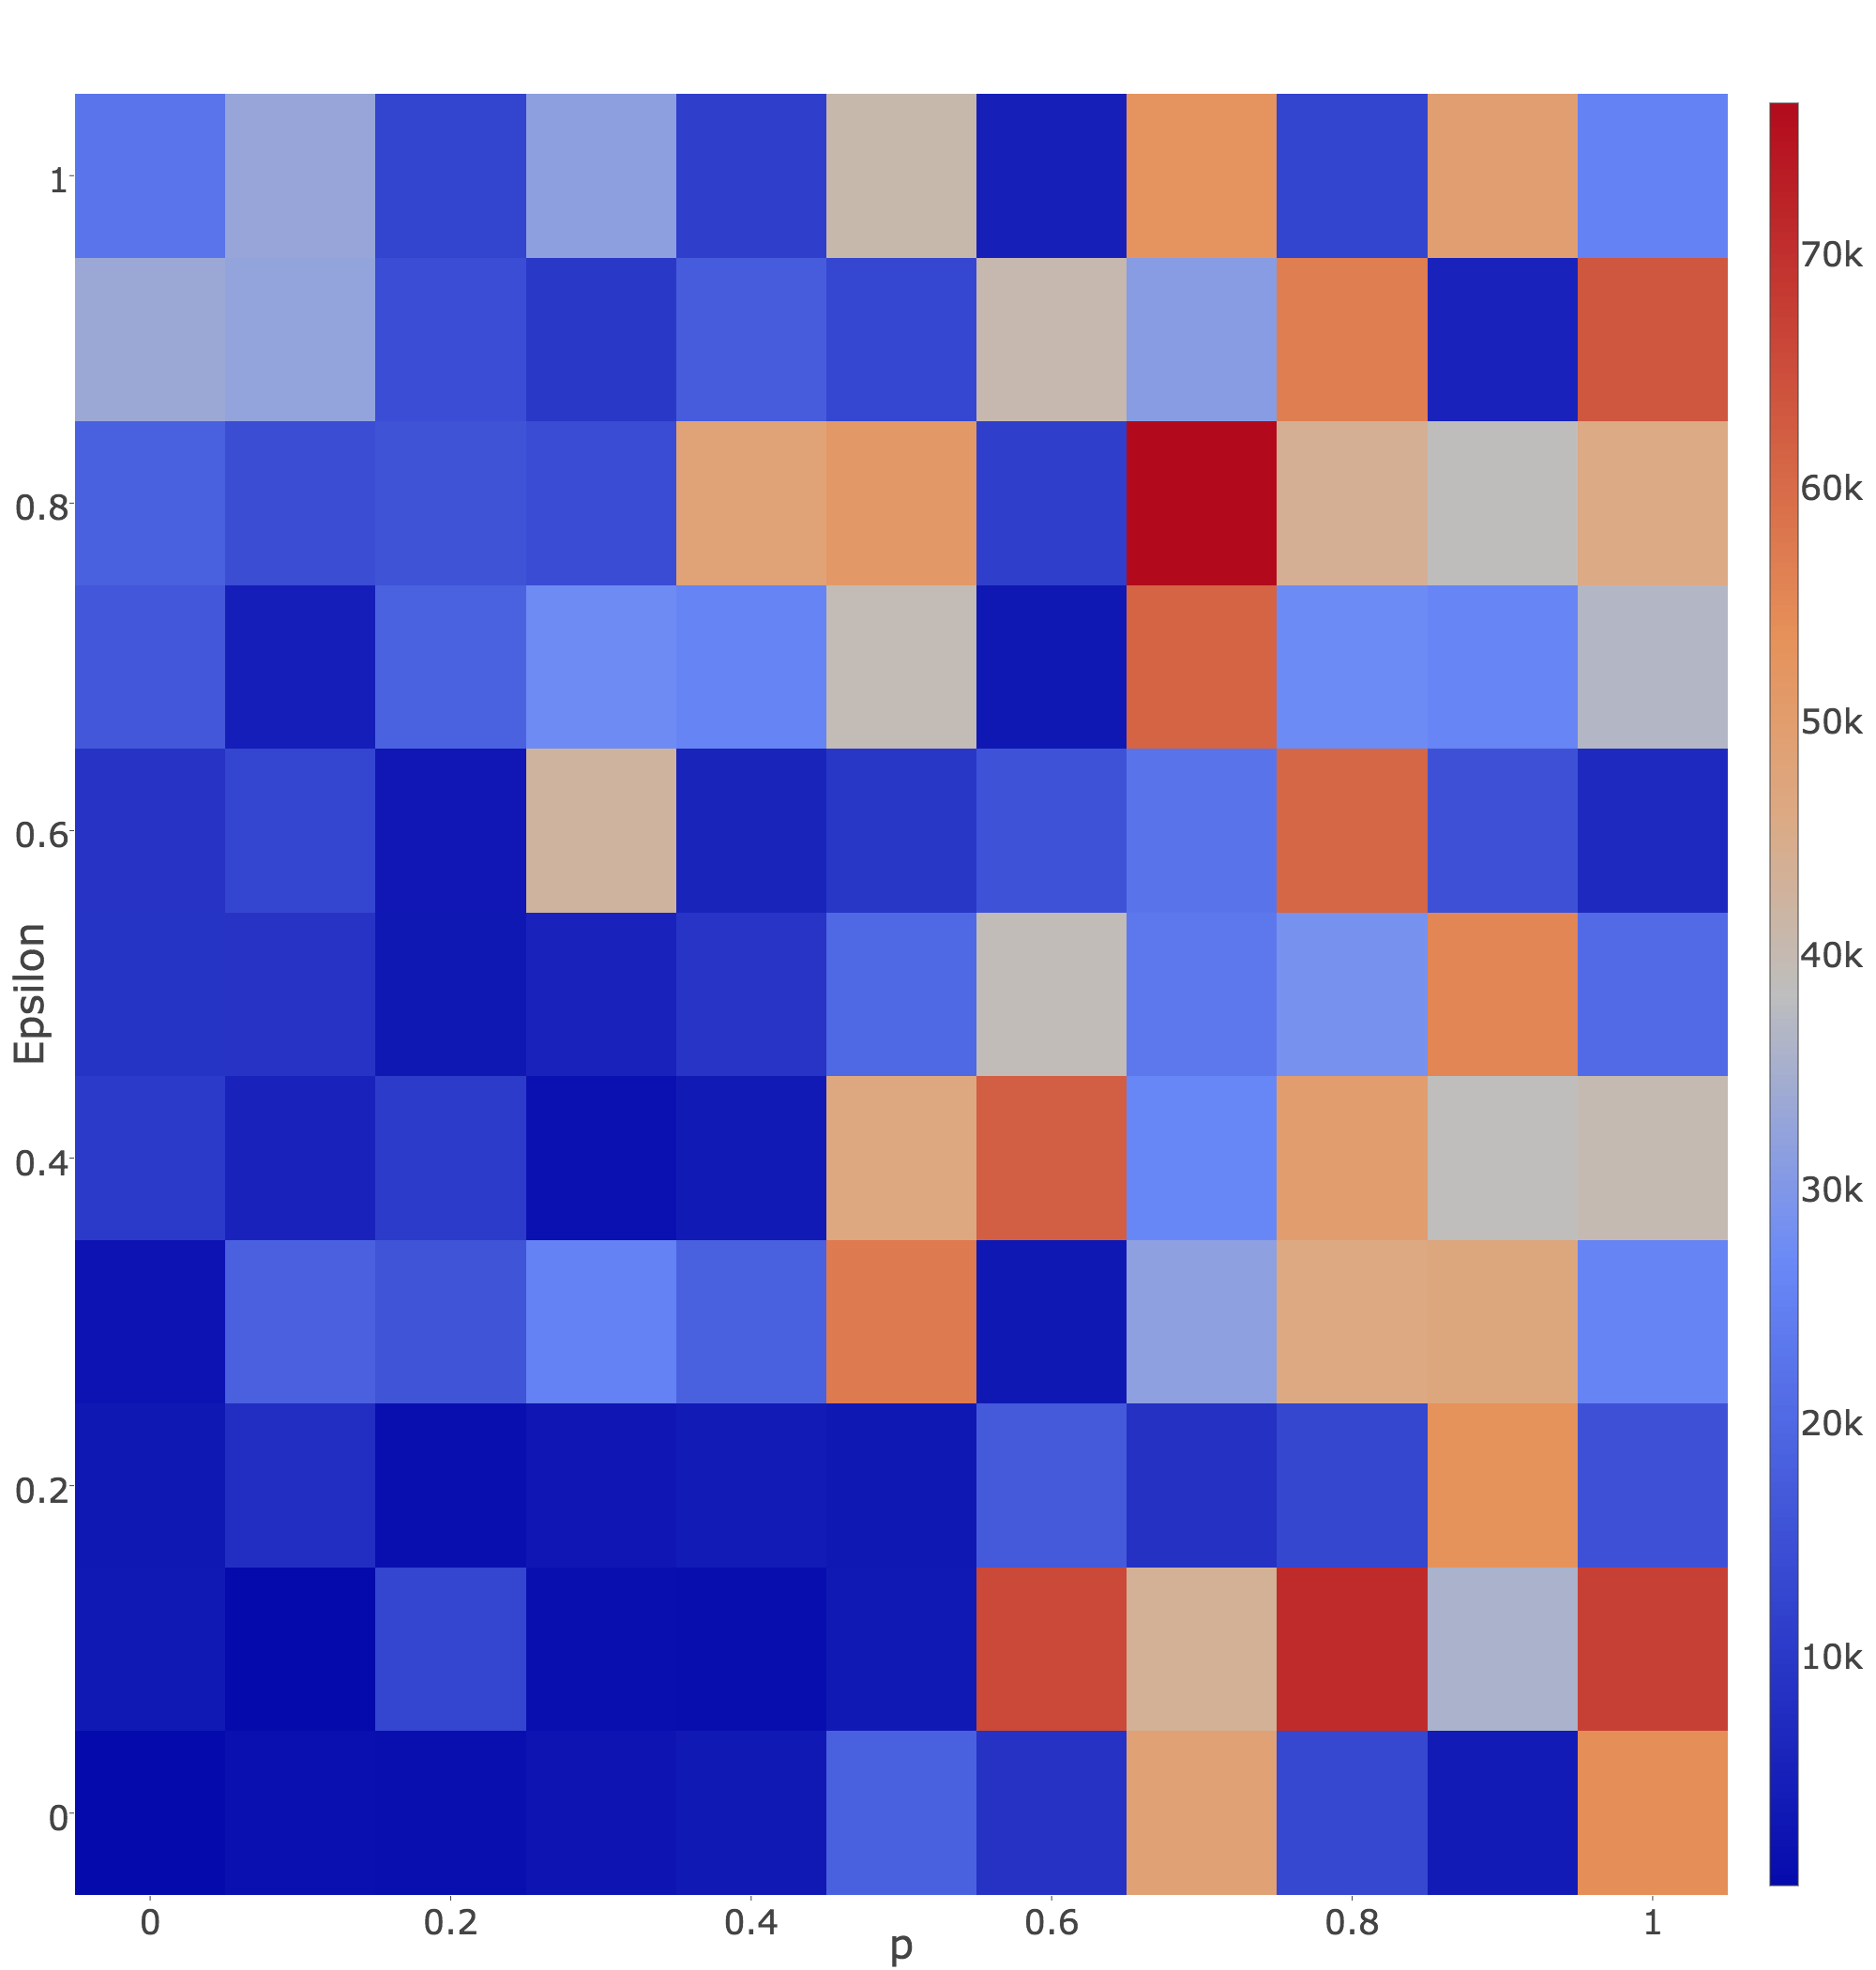
\includegraphics[width=.5\textwidth]{pics/medium03_heatmap}}{\centering\caption{Q-Learning scores for the medium map over a space of $p$ and $\epsilon$ values, visualized as a heatmap.}\label{fig:qlheatmap}}
    \end{floatrow}
\end{figure}
\begin{figure}[!htb]
    \begin{floatrow}
        \ffigbox{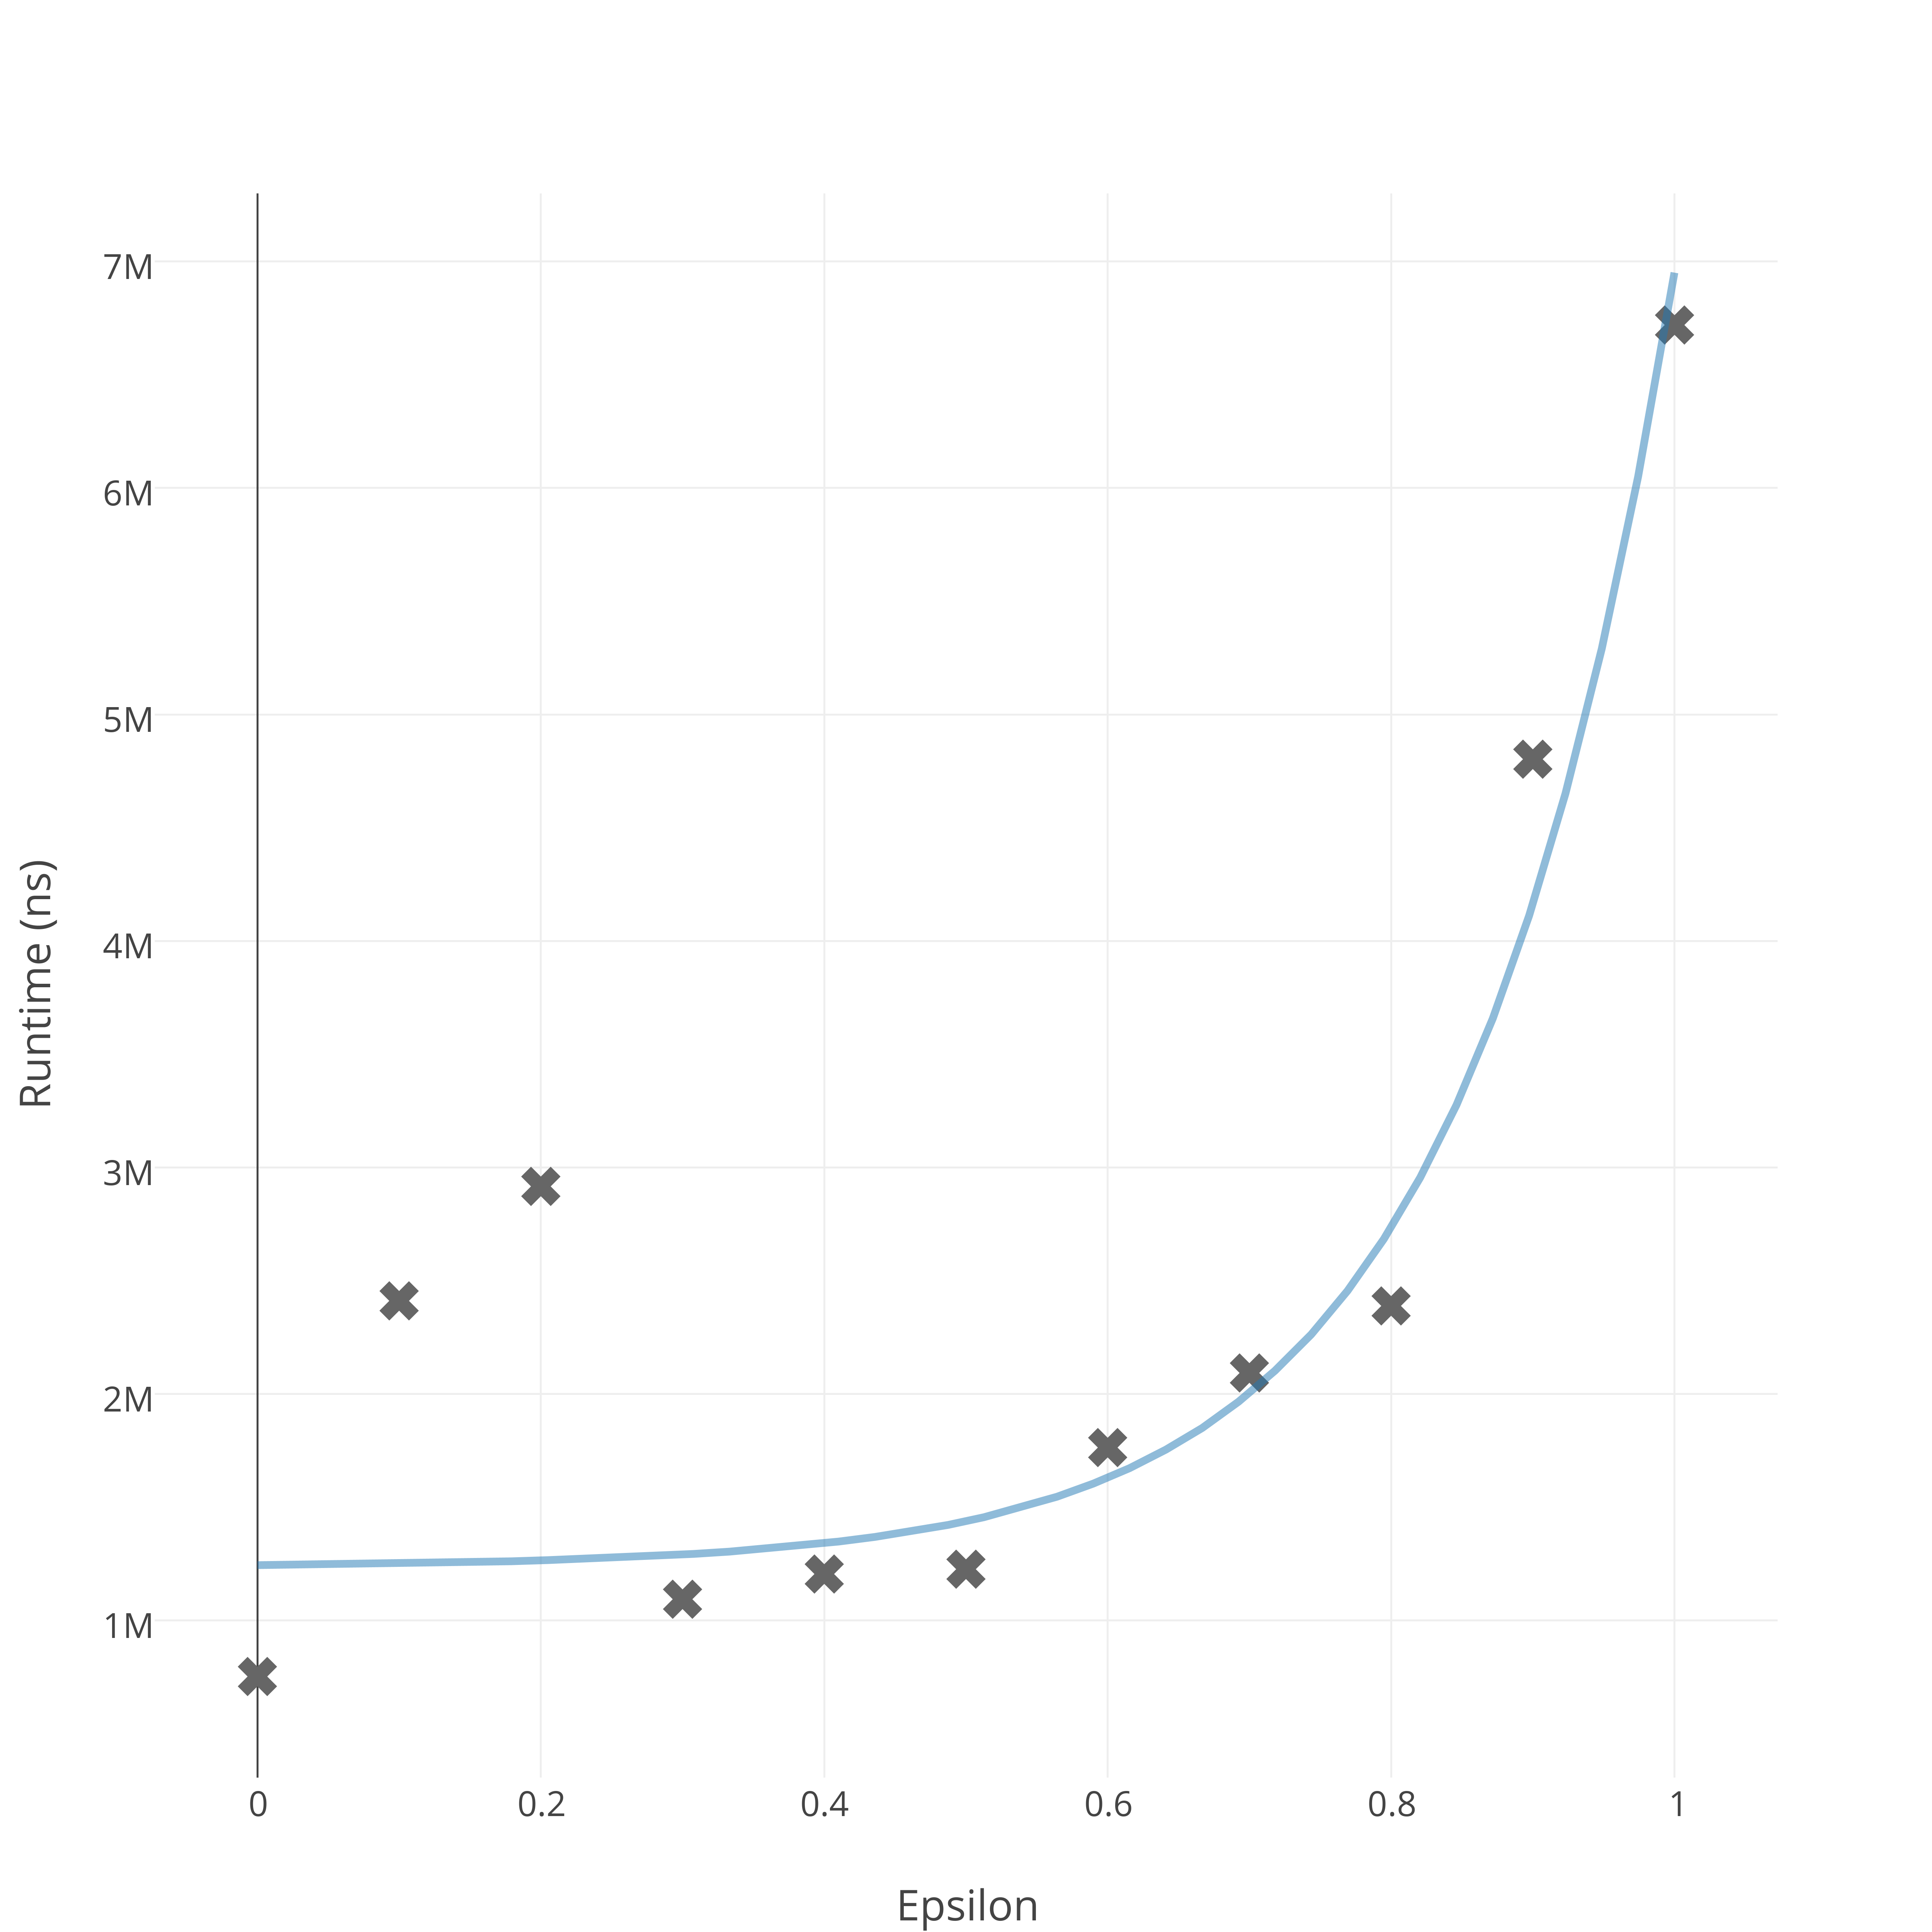
\includegraphics[width=.5\textwidth]{pics/runtimevsepsilon_medium}}{\centering\caption{$\epsilon$ vs runtime for the medium map for Q-learning. An exponential regression is superimposed on the graph.}\label{fig:qlruntimemedium}}
        \ffigbox{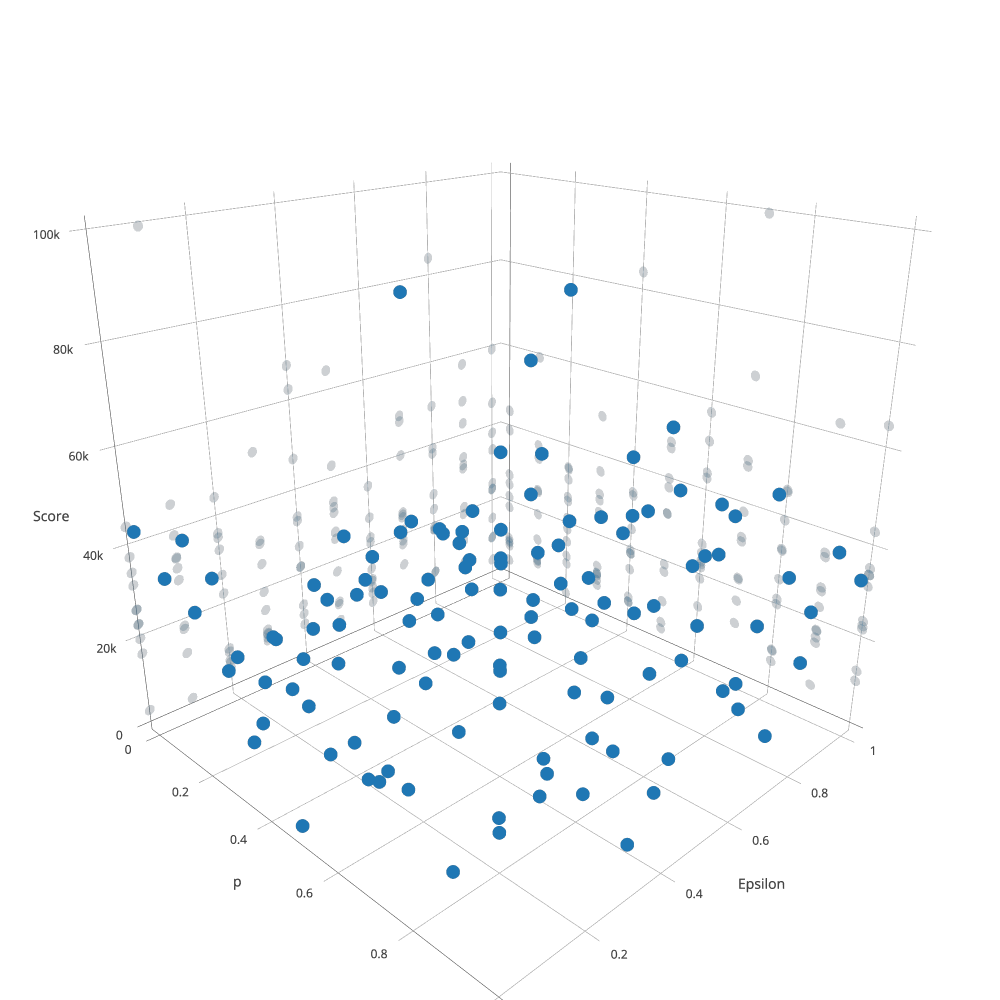
\includegraphics[width=.5\textwidth]{pics/QLearningBig}}{\centering\caption{Q-Learning scores for the big map over a space of $p$ and $\epsilon$ values, visualized as a 3D scatter plot.}\label{fig:qlscatterbig}}
    \end{floatrow}
\end{figure}

For the medium map (Figure \ref{fig:qlscatter}), there seems to be a linear relationship between the value function, $p$ and $\epsilon$. This effect is clearer on the heatmap (Figure \ref{fig:qlheatmap}). For the large map (Figure \ref{fig:qlscatterbig}), the relationship between $p$ seems to be very weakly linear with smaller $p$ values leading to slightly better policies. There appeared to be little relationship between $\epsilon$ and score.

Smaller $p$ values produced significantly better policies for both maps.\footnote{This may be hard to see on the scatterplot for the big map. Refer to the online interactive version to see this more clearly.} The relationship with $p$ was expected as that simply means less noise and more certainty in the transition model. Q-learning is especially sensitive to this given that is is a model-free learner.

Smaller $\epsilon$ produced slightly better policies in the medium map. This appears to indicate that for the smaller map, exploitation was suffient to produce good policies and that exploration was not neccessary. This makes sense given that there are few traps in the medium map. For the large map, values around 0.8 produces the best policies. For a large map with traps and multiple goals, exploration was advantageous as compared to strict exploitation. However, too much exploration produced worse results.

$\epsilon$ had a large impact on runtime - see Figure \ref{fig:qlruntimemedium}. There was an exponetial relationship between $\epsilon$ and runtime. This makes sense as exploration is about trading some controlled amount of runtime performance for some amount of exploration ($\epsilon$-greedy follows a Boltzmann distribution). However, this tradeoff is important to consider if the RL algorithm is running in a runtime-constrained environment.

\subsubsection{Comparision of Q-learning with model-based learners}

\noindent\textbf{Generated policies}\\
Q-learning on the medium map produced lower quality results as compared to model-based learners. This is expected as the model-based learners have information regarding the problem rewards and probabilities of the transition model. Q-learning at times produces strange results for certain states where many more iterations are required to converge.\\

\noindent\textbf{Runtime}\\
Q-learning takes significantly longer to converge when compared to model-based learners, both in terms of iterations as well as time. This makes sense as Q-learning has no starting knowledge regarding the problem. This demonstrates that Q-learning is trading learning time for a priori knowledge. These problems also had deterministic rewards - for situations with stocastic rewards, runtime could be pathologically worse as Q-learning would require repeated visits to a state.\\


\noindent\textbf{Effect of $p$}\\
Q-learning seems to be significantly more sensitive to the value of $p$ as compared to model-based learners. This makes sense as the Q-learner is effectively trying to learn the transition model probabiities through increased training time. Given a fixed number of iterations, it makes sense that Q-learning performance was heavily dependent on the choice of $p$.\\


\noindent\textbf{Exploration versus Exploitation}\\
For simpler maps with few traps, exploration was not that advantageous. For complex maps with many traps and multiple goals, increased exploration (to a point) produced better maps. Given a set MDP problem, the main lever for controlling Q-learning performance is the $\epsilon$ value. Deciding the amount of exploration is the key choice in a reinforcement learning problem. Choosing $\epsilon$ depends on how many states are in the MDP and how complex rewards are (more complex MDPs can benefit from increased exploration).


\subsection{Prioritized Sweeping}

Prioritized Sweeping is another model-based algorithm that has very interesting temporal properties as a result of its use of Bellman Backups. This paper explores the hyperspace of parameters, score and runtime. Figure \ref{fig:psscore}\footnote{For an interactive 3D scatter plot, see \url{https://plot.ly/~parasj/12.embed}} shows the relationship between score, $p$ and $\epsilon$. Figure \ref{fig:psruntime}\footnote{For an interactive 3D scatter plot, see \url{https://plot.ly/~parasj/13.embed}} explores the relationship between $p$, $\epsilon$ and runtime.

\begin{figure}[h]
    \begin{floatrow}
        \ffigbox{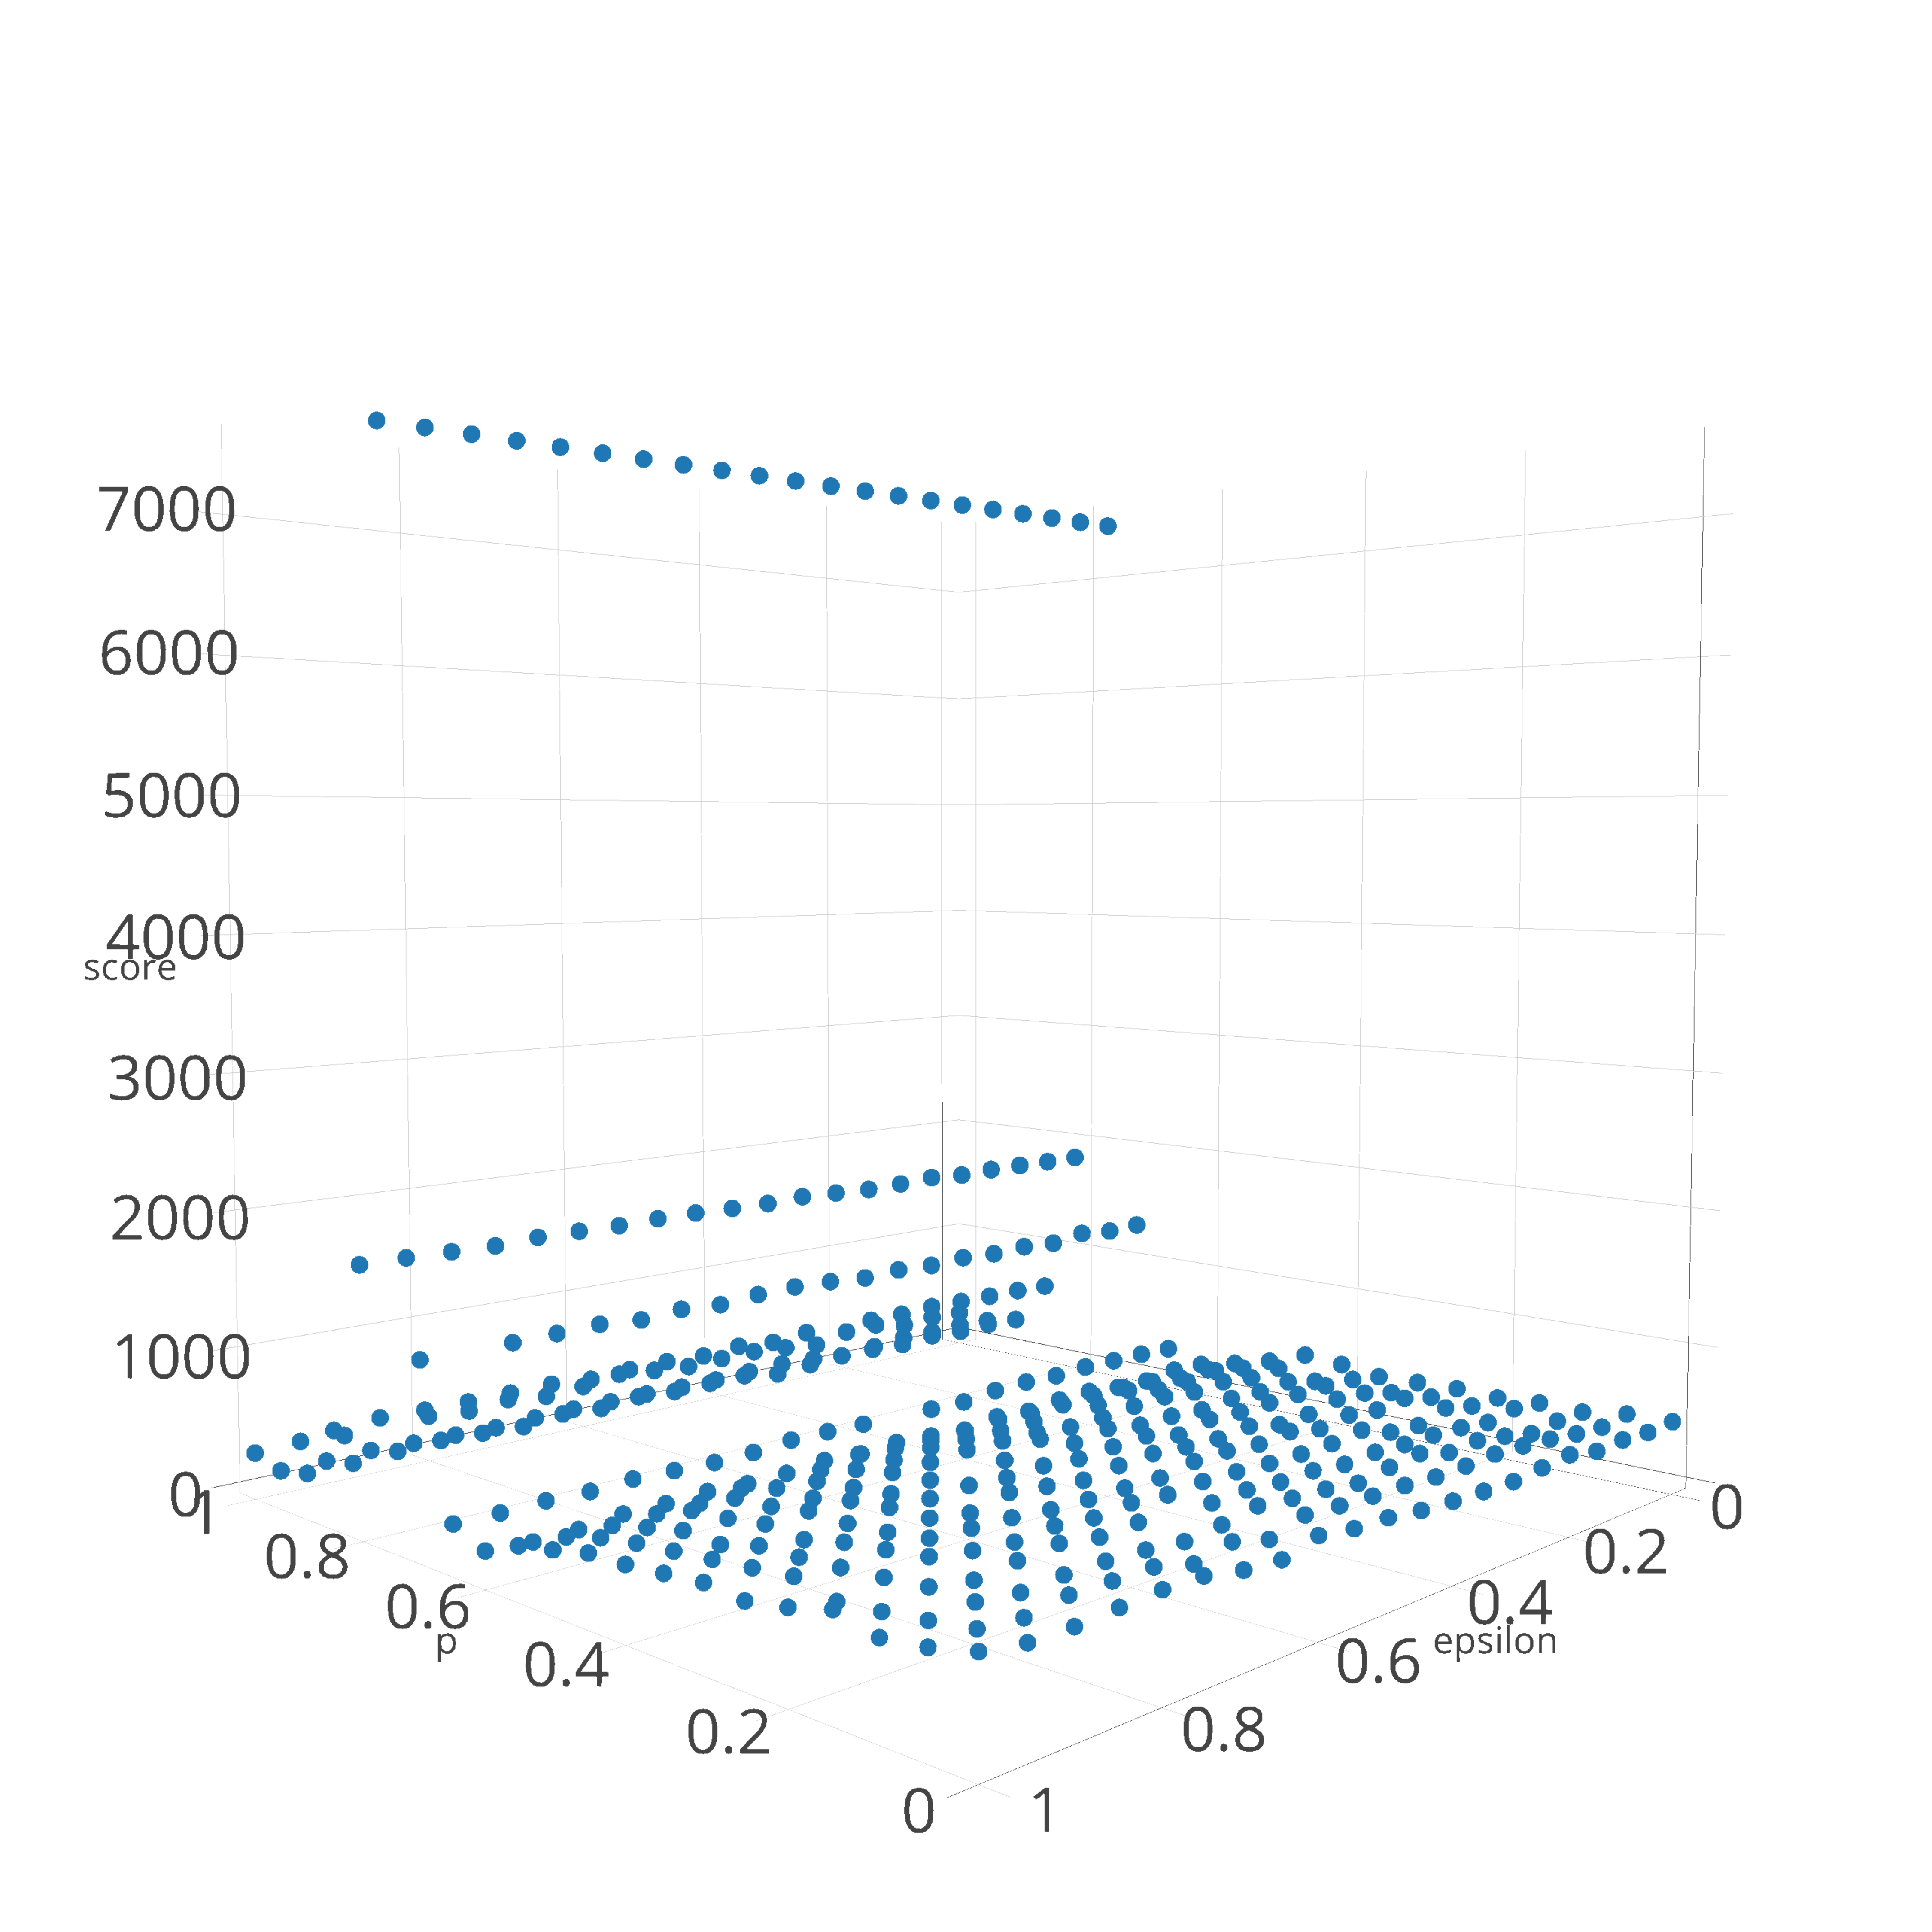
\includegraphics[width=.5\textwidth]{pics/p_epsilon_score}}{\centering\caption{Relationship between $p$, $\epsilon$ and score for the medium map with Prioritized Sweeping.}\label{fig:psscore}}
        \ffigbox{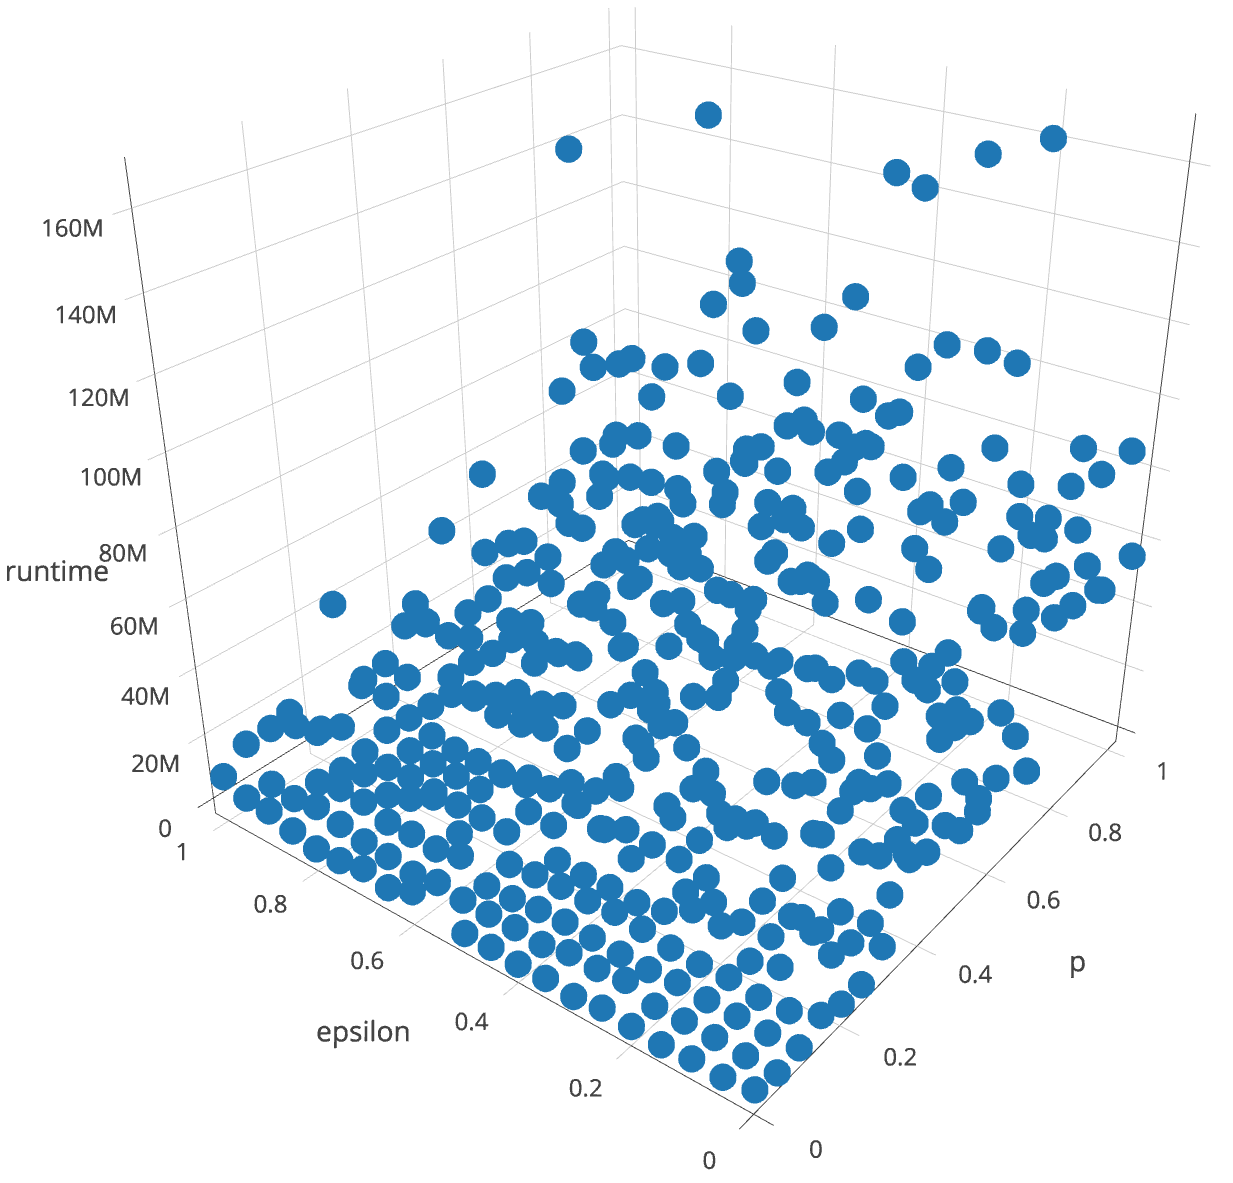
\includegraphics[width=.5\textwidth]{pics/PSruntime}}{\centering\caption{Relationship between $p$, $\epsilon$ and runtime for the medium map with Prioritized Sweeping.}\label{fig:psruntime}}
    \end{floatrow}
\end{figure}

\subsubsection{Effect of $p$ and $\epsilon$ on score}
Figure \ref{fig:psscore} is interesting as it seems $\epsilon$ has little impact on the score. However, it seems Prioritized Sweeping is very sensitive to the value of $p$. Moreover, it seems Priortized Sweepign has pathological cases near $p=0.7$ which is similar to Value Iterations pathological cases. I suspect this is for the same reason as Value Iteration where these cases are where the transition model is near random and therefore there is little that the algorithm can do to optimize a policy.

\subsubsection{Effect of $p$ and $\epsilon$ on runtime}
Figure \ref{fig:psruntime} is interesting when compared with the results from Q-learning. $\epsilon$ appears to have little impact on runtime which contrasts with Q-learning where it was $\epsilon$ that had an exponential correlation with runtime. However, unlike other model-based RL algorithms like Value Iteration and Policy Iteration, $p$ appears to exponentially correlate with runtime. As Prioritized Sweeping is a model-based learner, this was unexpected but makes sense as more uncertainty would lead to a tree-like effect when exploring the state space where exponentially more states need to be explored.



\section{Conclusion}
\subsection{Value Iteration}
Value iteration is effective overall and is reasonably quick at solving the optimal policy. It used an unexpected trick to optimize for situations where the probability of a succesful transition was low. However, value iteration took many iterations to converge and also had some pathological cases where the transition model was ambiguous. As value iteration is a model-based learner, it is only well suited to scenarios where the transition probability is known. Experiments showed that value iteration had good asymptotic performance for problems where the state space grew non-linearly.

\subsection{Policy Iteration}
Policy iteration worked reasonably well for the Gridworld MDPs. Policy iteration used the same trick as value iteration to produce similar optimal policies. It has lower constant-factor runtime constants so for smaller problems, it was faster than value iteration. However, its asymptotic runtime growth was worse than value iteration. Policy iteration did not seem to have as many pathological cases as value iteration which makes it well suited for ambiguous transition models. As it is a model-based learning algorithm like value iteration, it requires a priori knowledge of the state transition probabilities.

\subsection{Q-learning}
Q-learning trades some runtime performance for a priori information as it is a model-free learner and does not require the probability of a state transition. However, Q-learning takes many more iterations to converge as compared to a model-based algorithm and requires longer runtime. For Q-learning, results are very sensitive to the choice of $\epsilon$ which controls the exploitation-exploration tradeoff. Larger $\epsilon$ values cost exponentially more runtime but can produce more optimal policies for more complex MDPs. While Q-learning is less effective than value iteration or policy iteration, it does not require a priori knowledge of $p$.

\subsection{Prioritized Sweeping}
Prioritized sweeping was explored briefly to compare to the other model-based algorithms. It has performance characteristics similar to value iteration (which makes sense as it is essentially an incremental form of value iteration). Runtime is heavily dependent on $p$ but for MDPs which have low noise, prioritized sweeping can be an efficient way to solve for the optimal policy.




\end{document}